\title{A Brief Introduction to Symplectic Integrators in Numerical Analysis}
\author{
        Aditya Kumar \\        
        Department of Mathematics and Statistics\\
        McGill University, Montreal, QC\\
}
\date{December 20, 2012}

\documentclass[12pt]{article}

\usepackage{indentfirst}
\usepackage{hyperref}
\usepackage{graphicx}
\usepackage{parskip}
\usepackage{amssymb} %math symbols
\usepackage{amsmath} %math stuff
\usepackage{mathtools}
\usepackage{verbatim}
\usepackage{mathrsfs}
\usepackage{fullpage}
\usepackage{amsthm}

\setlength{\parindent}{1cm}

\begin{document}
\maketitle

\begin{abstract} 
Symplectic Integrators is a specific numerical integration scheme that nearly conserves total energy of a dynamical system and can help understand the evolution of a dynamical system for very large time-scales. In this project, I present a basic introduction to some properties of symplectic integrators. By way of the example of the simple harmonic oscillator (s.h.o.) differential equation, I will demonstrate the properties of symplectic integrators of first-, second- and fourth-order, comparing them to the more commonly available numerical integration schemes such as explicit Euler, and Runge-Kutta second order/fourth order methods.  
\end{abstract}

\section{Introduction}
When studying dynamical systems, it is sometimes necessary to study the behavior of the system for long time scales, thus aiding in understanding the general evolution of the system. In Particular, if the system is described by a time-independent Hamiltonian, it can be seen that using symplectic integration methods can be superior to general purpose ordinary differential equation (o.d.e.) numerical schemes. It will be shown that general purpose o.d.e. solvers such as explicit euler and various order Runge-Kutta methods do not conserve total energy. If we apply such ode methods to the simple harmonic oscillator (s.h.o.), the computed energy value drifts from the exact energy solution, providing surprisingly poor results. Another reason for studying symplectic integrators also comes from the fact that the exact flow of Hamilton's equations is a symplectic map, and therefore when studying dynamical system described by a Hamiltonian one can find that numerically a better performance could be anticipated if using a symplectic integrator. I will introduce a few simple symplectic integration schemes and show that these algorithms do not exhbit the problem of energy drift.\\\\
\indent The symplectic integrator is a specific type of geometric integrator numerical scheme. Such algorithms are constructed so that the underlying geometric properties that are inherent to the system are preserved. Symplectic methods are named so due to the idea that when applied to problems in Hamiltonian mechanics, the algorithms preserve the linear symplectic structure inherent in the phase space representation of the dynamics of the system. The study of such algorithms was first done by Volgelaere \cite{RV}. Further work on such algorithms was independently done by Ruth whilst studying symplectic integrators and numerical integration schemes applied to the dynamics of particle accelerators \cite{RR}. Afterwards, symplectic integrators were studied in fields such as celestial mechanics, classical mechanics, and molecular dynamics \cite{MPS}. It was observed that for the symplectic integrators, the error in the total energy remains bounded over significant times. Hence, further research in symplectic integrators was initiated due to the relative simplicity of the algorithms and the boundedness of the error in energy.\\\\
\indent In this paper, I will be studying first-, second- and fourth-order symplectic integrator schemes, while comparing these schemes to the general purpose o.d.e. numerical schemes. The particular problem that will be modeled by these numerical schemes is the simple harmonic oscillator, enabling a geometric, analytic, and numerical perspective of the numerical methods. The advantage of this one-dimensional example is that the dynamics associated
with the numerical algorithms can be solved analytically, allowing for a direct analysis of the numerical solutions. I will show how the numerical algorithms attempt to conserve total energy and illustrate how the symplectic algorithms preserve the symplectic structure of phase space. In Sec. 2, I will briefly discuss setting for symplectic integrators, the notion of a linear symplectic structures and the idea of a symplectic map. In Sec. 3-5, I will discuss the symplectic Euler method compared with explicit Euler method, the symplectic velocity Verlet method compared with MATLAB ode23 solver, and symplectic fourth-order Forest-Ruth method compared with MATLAB ode45 solver.

\section{Brief Overview of Symplectic Maps and Symplectic Integration}

Before jumping into the general setting of symplectic integrators via Hamiltonian mechanics, the notion of ``symplectic'' should be somewhat defined. Symplectic integrators rely on symplectic geometry, which can be studied in a physical setting by constructing certain dynamical systems, particularly in classical mechanics, using Hamilton's equations. In studying dynamical systems from Hamiltonian differential equation framework, one can appreciate and use the underlying linear symplectic geometric framework that is inherent to the dynamical system. A symplectic map can be used to describe the mathematics that is taking place for the symplectic integrator. A symplectic map is a map which preserves the sum of areas projected onto a set of planes for a particular set of coordinates (mainly the Hamiltonian coordinate system). Such a map is a generalization of an area-preserving map. Rigorously speaking, the map is a real-linear map $T$ that preserves the symplectic form $f$ such that
\[f(Tx,Ty)=f(x,y)\]
for all $x,y$. This particular map is part of the underlying symplectic structure for Hamiltonian mechanics. \\\\
\indent The Hamiltonian mechanics framework is constructed in a $2n$-dimensional set of points (called a phase space) with coordinates $(q_i,p_i) \text{for} i=1,2,...n$. As stated in \cite{DR} ``For a particular system, the dynamics is defined once a Hamiltonian function $H(q,p)$, is specified. The phase space represents a possible state of the system. As the system evolves from a given set of initial conditions, the associated states form a curve in phase space whose tangent vector at each point is $(H_{p_i},-H_{q_i})$. The identification of the tangent vector to the curve of states with the vector $(H_{p_i},-H_{q_i})$,
\[\frac{dq}{dt}=H_{p_i}, \;\;\; \frac{dp}{dt}=-H_{p_i}\] 
which is the geometric interpretation of Hamilton's equations.''It is noted that for $(q_i,p_i)$, if we let $i=1$, this will represent a system with single degree of freedom. I will not be delving further into the symplectic geometries that govern Hamiltonian systems, and particular rigorous construction of phase flow, as this paper is mainly about numerical results. Rather, I direct readers to \cite{DR}, \cite{MPS} which develop the mathematics quite nicely and have plenty of references to texts in symplectic geometry applied to mathematical analysis of symplectic integrators.  Now using this framework, one can construct conditions for an algorithm to be symplectic (area-preserving). To do this, let us suppose that we have a square on the phase space $(q,p)$, with the four corners of the square having coordinates (q,p),(q+$dq$,p),(q,p+$dp$),(q+$dq$,p+$dp$), labelled 1,2,3,4, which represent a particle at time $t$. Then, at a later time $t'$ each of these four points will have changed, to form the corners of a parallelogram. Let the area of the parallelogram be $dA'$. An important theorem called Liouville's phase space theorem essentially states that the areas of the square at time $t$ and the subsequent evolution of the square over time $t'$ to the parallelogram are equal, i.e.
\[dA'=dA\]
where $dA$ is the area of the square at time $t$. Now $(q,p)$ transforms to $(q',p')$ where $q'$ and $p'$ are some functions of q, and p, i.e.
\[q'=Q(q,p)\]
\[p'=P(q,p)\]
which in this framework is the resulting symplectic (area-preserving) map. Since the area preserving property is an exact feature of the equations, it is desirable that a numerical approximation perserve it. Now to find a condition that will allow us to check if a particular numerical scheme is symplectic, we just need to compute the area $dA'$ and set it equal to $dA=dq\;dp$. The area of $dA'$ is given by
\[dA'=|d\vec{e_1}'\times d\vec{e_2}'|\]
where $d\vec{e_1}'$ represents one side of the parallelogram $1\rightarrow4$ and $d\vec{e_2}'$ the other side $1\rightarrow2$. Now the components of $d\vec{e_1}'$ are just the changes in $q'$ and $p'$ when $q$ is change by $dq$ but $p$ is fixed, i.e.
\[d\vec{e_1}'=\left(\frac{\partial q'}{\partial q}\hat{q} + \frac{\partial p'}{\partial q}\hat{p} \right)dq\]
and similarly,
\[d\vec{e_2}'=\left(\frac{\partial q'}{\partial p}\hat{q} + \frac{\partial p'}{\partial p}\hat{p} \right)dp\]
It is known that the area of the parallelogram can be represented as a determinant, thereby having
\[dA'=\text{det}\;J\;dA\]
where $J$ is 
\[J=\left(
  \begin{array}{c c}
     \frac{\partial q'}{\partial q} & \frac{\partial q'}{\partial p} \\\\
     \frac{\partial p'}{\partial q} & \frac{\partial p'}{\partial p}
  \end{array} \right)\]
Thus, det$J$ is the Jacobian of the transformation from $(q',p')$ to $(q,p)$ which occurs when you do change of variables in an integral. Hence a symplectic algorithm has 
\[\text{det}\;J=1\]
Now we can set up the main problem that we will use to compare numerical schemes. For the s.h.o. with the Hamiltonian $H(q,p)=\frac{1}{2}(q^2+p^2)$ we have the coupled first order differential equations:
\[\frac{dq}{dt}=H_p=p\]
\[\frac{dp}{dt}=-H_q=q\]
that can be solved for analytically, and thus whose solution gives the phase flow
\[q(t)=cos(t)+sin(t)\]
\[\;\;\;p(t)=-sin(t)+cos(t)\]
with the particular initial conditions being $q(0)=1$ and $p(0)=0$ and setting $k=1$ and $m=1$. In general, a method is $n$th-order for a differential equation $y'=f(y), y(t_0)=y_0$, if $y_1-y(t_0+\Delta t)=O(\Delta t^{n+1}$ as $\Delta t \rightarrow 0$, where $y_1$ is the result of applying the particular numerical method to the initial state $y_0$ for one time step.


\section{First-Order Methods: Explicit Euler and Symplectic Euler}
We start with the most familiar first-order method, the classic explicit Euler method:
\[q_{i+1}=q_i+p_i\Delta t,\]
\[p_{i+1}=p_i+F_i\Delta t\]
where, for the s.h.o., $F_i=(1)(\frac{dp}{dt})=-q_i$. We write the explicit Euler method in terms of Hamilton's equations,
\[\left (\begin{matrix}
  q_{i+1}  \\
  p_{i+1} 
 \end{matrix}\right)=
\left(\begin{matrix}
  1 & \Delta t \\
  -\Delta t & 1 
 \end{matrix}\right)
\left(\begin{matrix}
  q_i  \\
  p_i 
 \end{matrix}\right)\]
which is the first order approximation of the exact solution
\[\left (\begin{matrix}
  q_{i+1}  \\
  p_{i+1} 
 \end{matrix}\right)=
\left(\begin{matrix}
  cos(\Delta t) & sin(\Delta t) \\
  -sin(\Delta t) & cos(\Delta t) 
 \end{matrix}\right)
\left(\begin{matrix}
  q_i  \\
  p_i 
 \end{matrix}\right)\]

To see why the explicit Euler method is not symplectic, we check symplectic map condition, i.e., check to see if the Jacobian transformation is equal to unity. We get
\[\left(\begin{matrix}
  1 & \Delta t \\
  -\Delta t & 1 
 \end{matrix}\right)=1+{\Delta t}^{2}\]
which is not equal to unity, hence the explicit Euler method is not symplectic. Now we move onto the numerical results of the explicit Euler for the s.h.o.
\begin{figure}[h!]
\centering
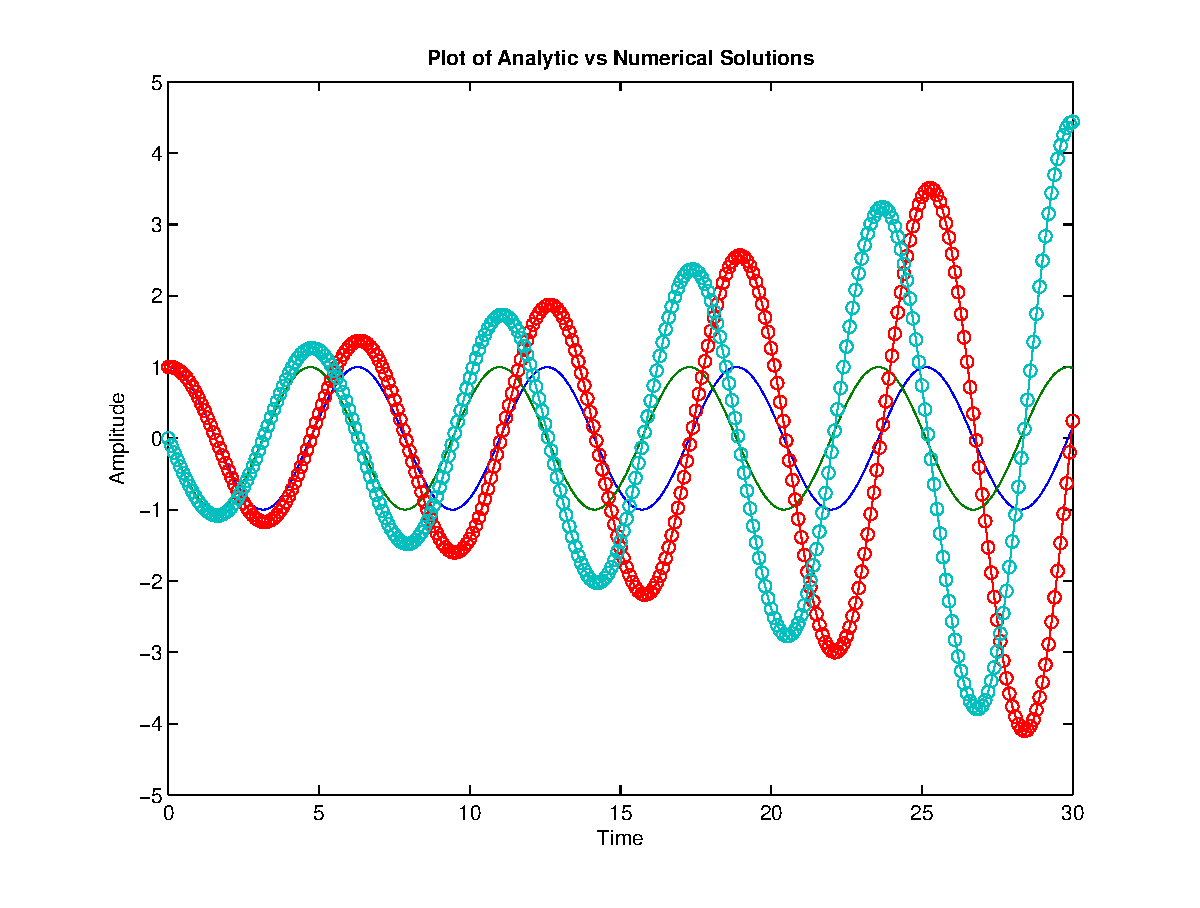
\includegraphics[width=0.675\textwidth]{ExplicitEulerPlotOfAnalyticVsNumSoln}
\caption{Plot of the analytic solution of the s.h.o. q(t) and the explicit Euler numerical solution. q(t) is represented by the green and dark blue oscillations that are constant in amplitude over time. The red and the light blue oscillations that are growing in amplitude over time represent the explicit Euler method.}
\end{figure}
\\\\
\indent We see in Figure 1 that the numerical approximation done by the explicit Euler method starts to rapidly grow over long periods of time, continuously diverging away from the exact solution which has a constant amplitude over time. For a short time step, the explicit Euler method does well in maintaining close approximation to the exact solution. We computed that the Jacobian is $1+{\Delta t}^{2}$ for the explicit Euler, which can be seen as the factor for each iteration at which the amplitude of the oscillations is increasing montonically. 
\\\\
\indent In Figure 2 and Figure 3 we have the numerical approximations of the phase space portrait and of the energy. For the phase space portrait, we see that the explicit Euler shows the phase space trajectory is increasing and spiraling outwards. The area in the phase space increases monotonically by a factor of $1+{\Delta t}^{2}$ with each iteration as the phase space trajectory spirals outward. For the energy graph, we see that the energy of the s.h.o. should be constant, yet there is some artificial excitation in the explicit Euler method that shows the energy of the s.h.o. monotonically increasing again with a factor of $1+{\Delta t}^{2}$. \\\\\\
\begin{figure}[h!]
\centering
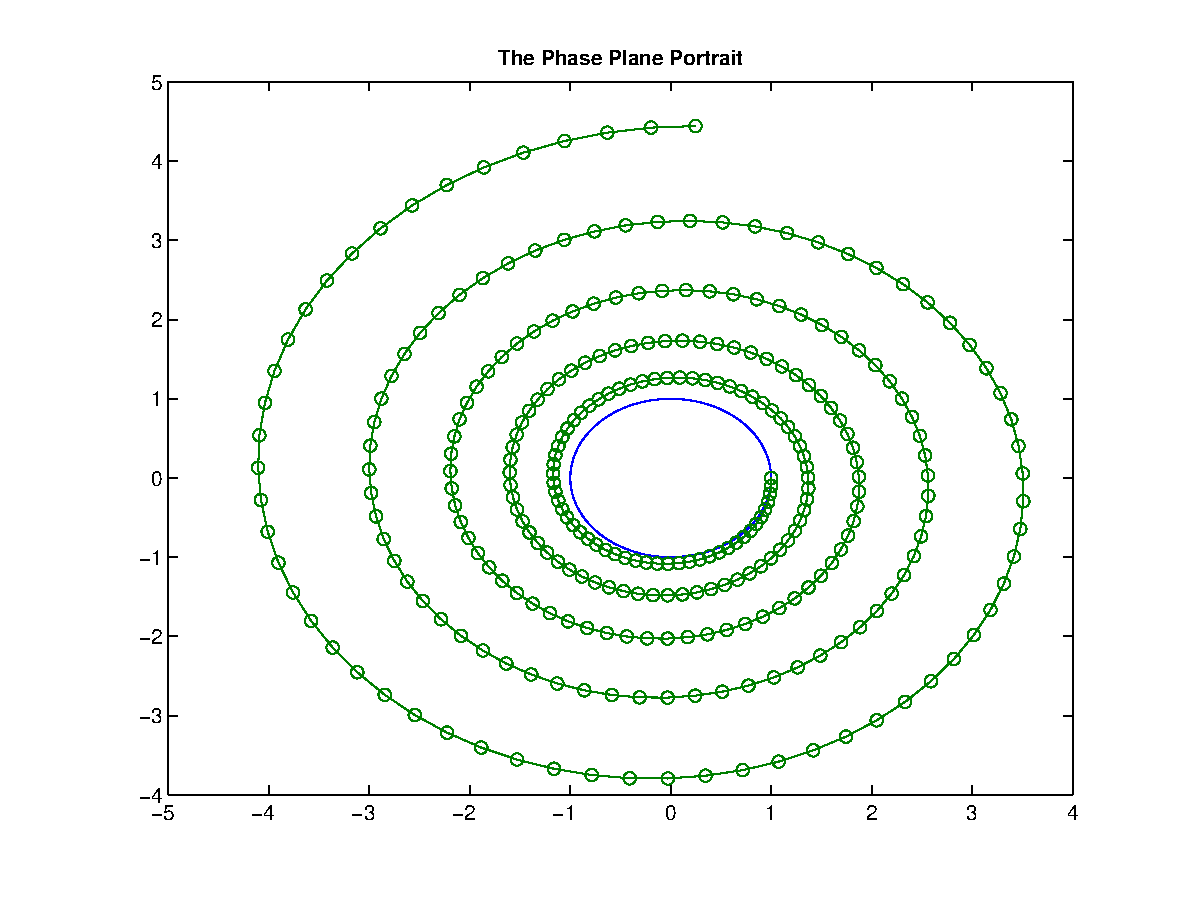
\includegraphics[width=0.675\textwidth]{ExplicitEulerPhasePlanePortrait}
\caption{Plot of the position-momentum phase space of the explicit Euler in green and the exact phase space in blue, which is the exact movement of the s.h.o.}
\end{figure}
\begin{figure}[h!]
\centering
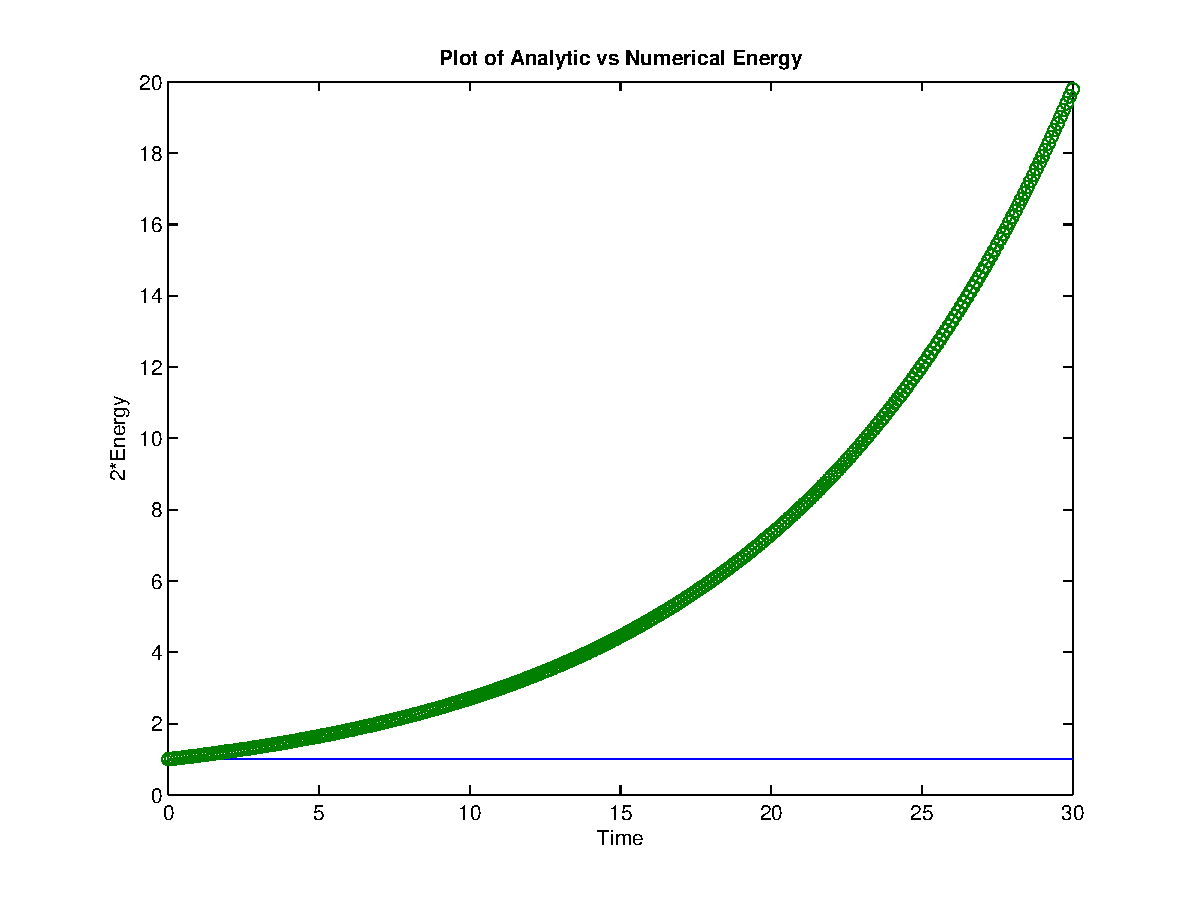
\includegraphics[width=0.675\textwidth]{ExplicitEulerAnalytVsNumEnergyPlot}
\caption{Plot of the total energy multiplied by 2 of the s.h.o. in which exact energy is blue and the energy computed by explicit Euler is in green.}
\end{figure}
\indent Now we compare this with the results of the symplectic Euler. The symplectic Euler is a combination of implicit and explicit first-order methods (again, making it first-order). So, if we write the momentum $p$ in implicit form and position $q$ in explicit form we get that for any Hamiltonian that is time-independent, $H(q,p)$,
\[q_{i+1}=q_i+\frac{\partial H(q_i,p_{i+1})}{\partial p}\Delta t\]
\[p_{i+1}=p_i-\frac{\partial H(q_i,p_{i+1})}{\partial q}\Delta t\]
Then, for the s.h.o. the symplectic Euler scheme is
\[\;\;\;q_{i+1}=q_i+p_{i+1}\Delta t\]
\[p_{i+1}=p_i-q_i\Delta t\]
Verifying the condition of symplecticity, we see that
\[q_{i+1}=q_i+(p_i-q_i\Delta t)\Delta t\]
\[\;q_{i+1}=(1-{\Delta t}^{2})q_i+p_i\Delta t\]
\[p_{i+1}=p_i-q_i\Delta t\;\;\;\;\;\;\;\;\;\;\;\;\;\;\]
\[\left (\begin{matrix}
  q_{i+1}  \\
  p_{i+1} 
 \end{matrix}\right)=
\left(\begin{matrix}
  1-{\Delta t}^{2} & \Delta t \\
  -\Delta t & 1 
 \end{matrix}\right)
\left(\begin{matrix}
  q_i  \\
  p_i 
 \end{matrix}\right)\]
indeed the determinant of the Jacobian is equal to unity and thus the method is symplectic. Now we move onto the numerical results from the symplectic Euler method while comparing it to the explicit Euler method results above.
\begin{figure}[h!]
\begin{minipage}[b]{0.45\linewidth}
\centering
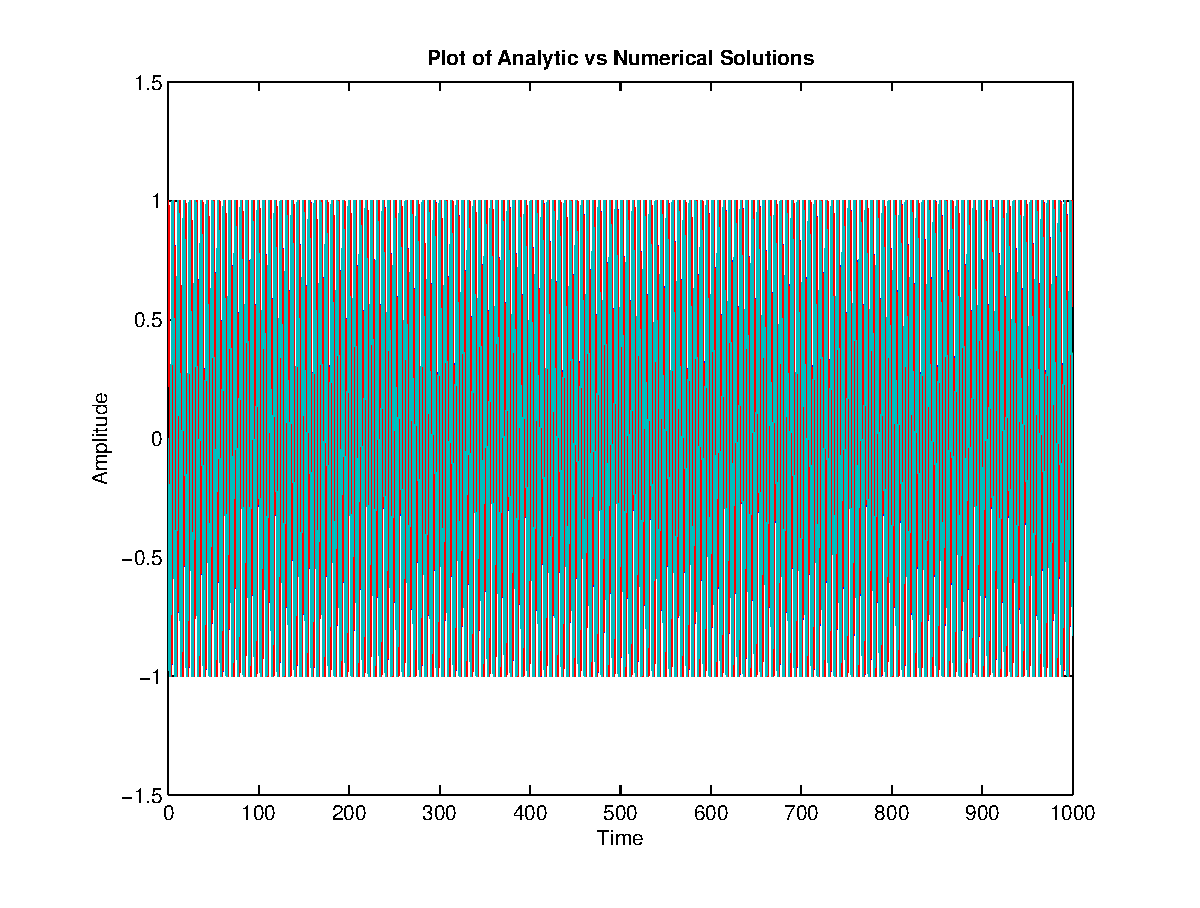
\includegraphics[width=\textwidth]{SymplecticEulerPlotofAnalyVsNumSoln}
\caption{Plot of the analytic solution $q(t)$ of the s.h.o. in green and dark blue and plot of the symplectic Euler numerical solution in red and light blue.}
\label{fig:figure4}
\end{minipage}
\hspace{0.5cm}
\begin{minipage}[b]{0.45\linewidth}
\centering
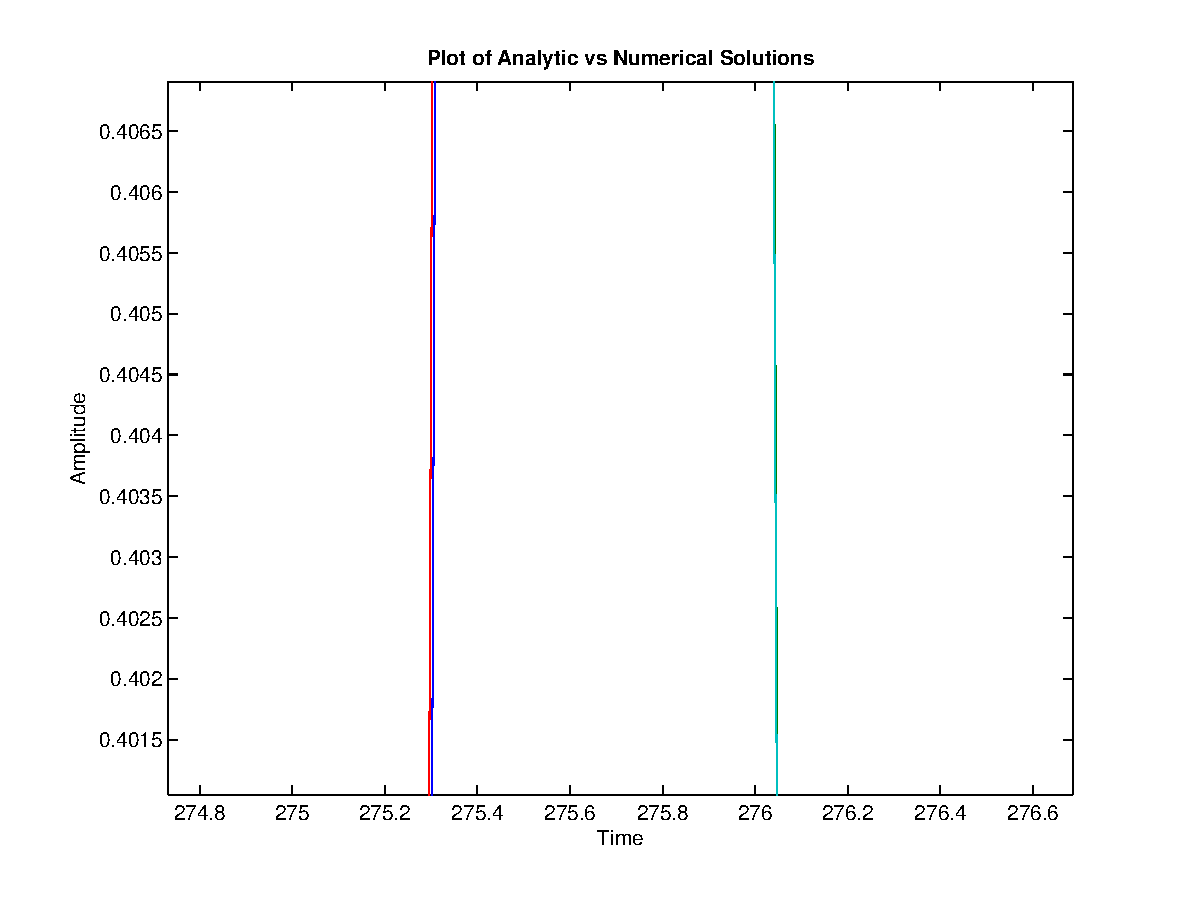
\includegraphics[width=\textwidth]{ZoomedInSymplecticEulerPlotofAnalyVsNumSoln}
\caption{A close-up of the plot in Figure 4. Here we can see the strong approximation of the symplectic Euler method in relation to the exact solution.}
\label{fig:figure5}
\end{minipage}
\end{figure}
\\\\\indent We see in Figure 4 and Figure 5 that the numerical approximation done by the symplectic Euler method is very close to the exact solution. For the symplectic Euler method, the amplitude of the oscillations over time is constant, like the exact solution. Figure 5 shows that even though the approximation is quite good, it is not exact. It seems that the symplectic Euler approximates the s.h.o. by essentially solving a small perturbated s.h.o. system that is quite similar to the s.h.o. This means that the symplectic Euler has solved a modified Hamiltonian that closely represents the original Hamiltonian. As we take smaller and smaller time steps, the scheme will approach the exact Hamiltonian of the s.h.o. we started with. 
\begin{figure}[h!]
\begin{minipage}[b]{0.45\linewidth}
\centering
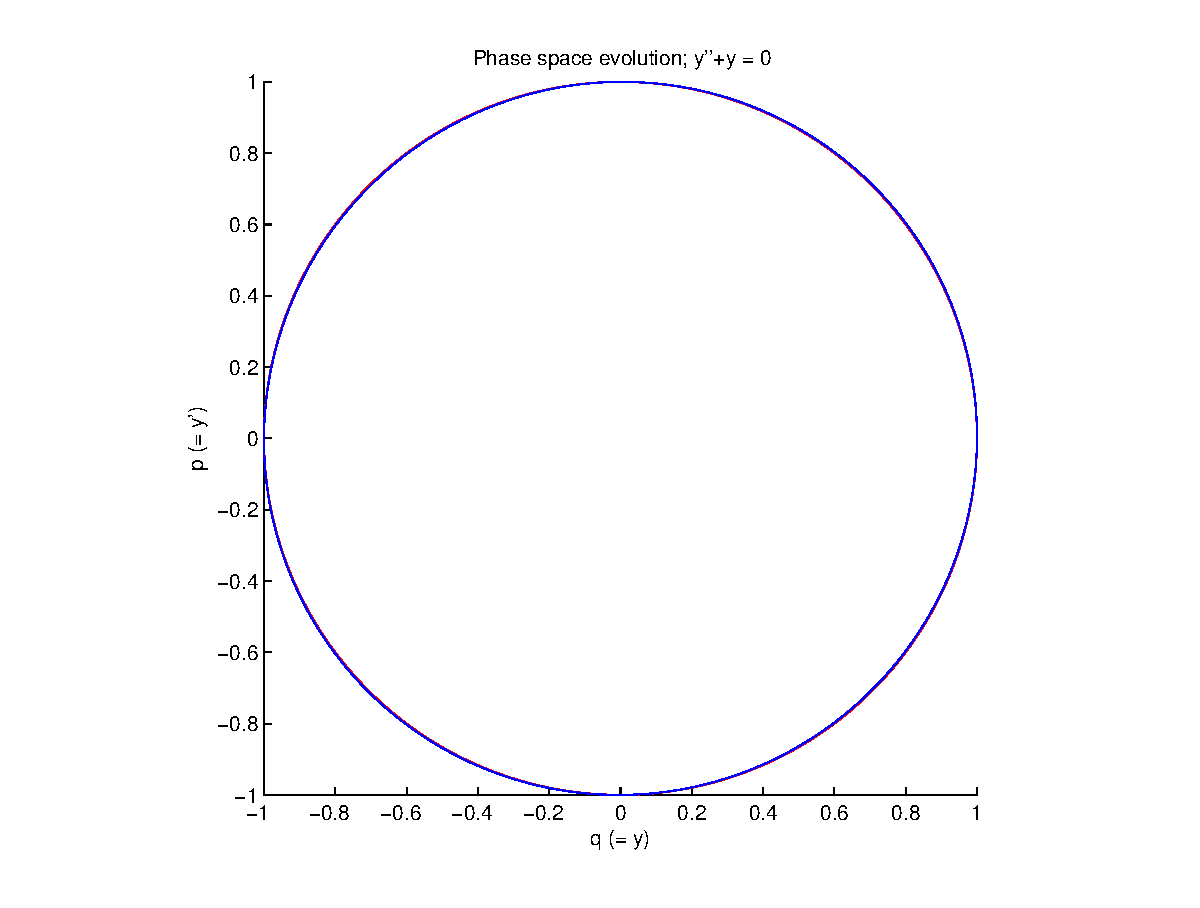
\includegraphics[width=1.1\textwidth]{SymplecticEulerPhaseSpacePlot}
\caption{Plot of the position-momentum phase space of the symplectic Euler in red and the exact phase space in blue, which is the exact movement of the s.h.o.}
\label{fig:figure6}
\end{minipage}
\hspace{0.5cm}
\begin{minipage}[b]{0.45\linewidth}
\centering
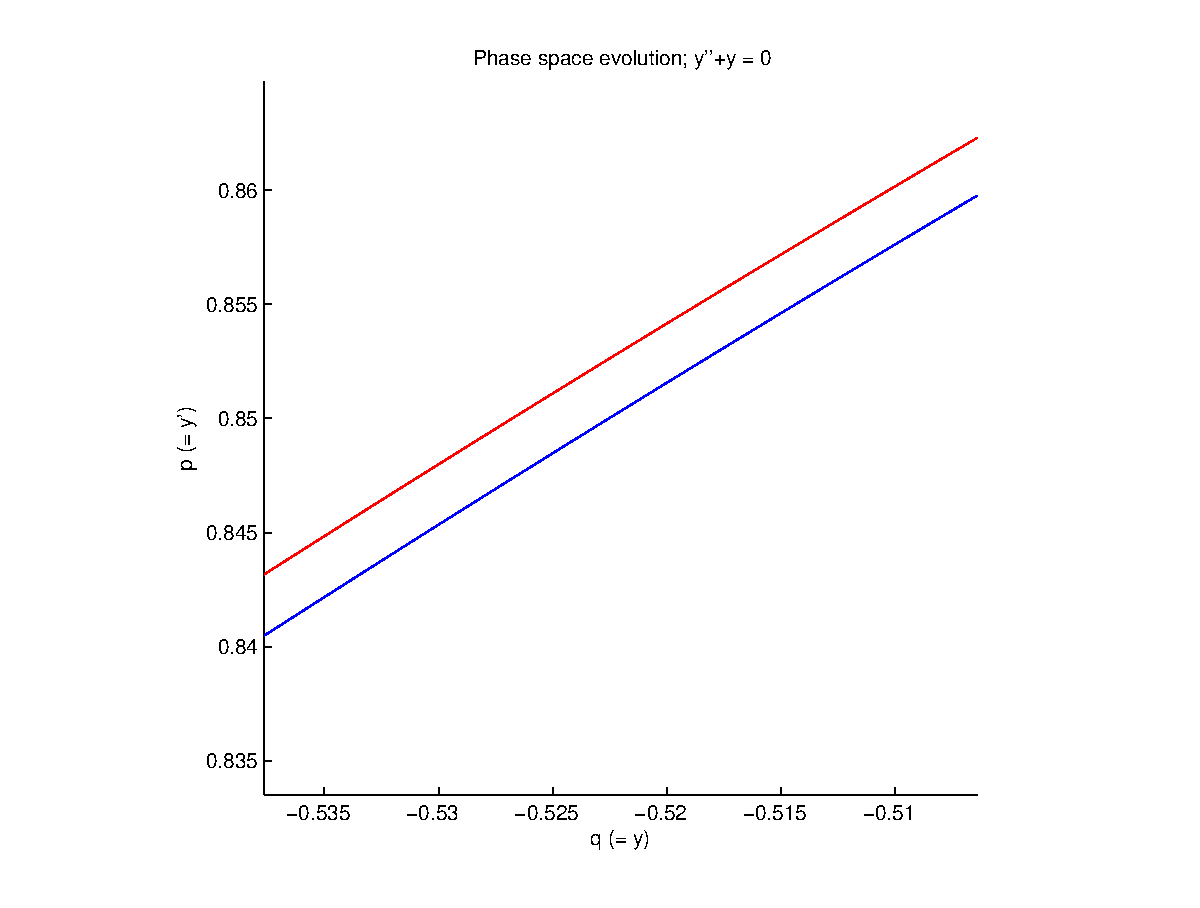
\includegraphics[width=1.1\textwidth]{ZoomedInSymplecticEulerPhaseSpacePlot}
\caption{A close-up of the plot of the position-momentum phase space showing the very slight difference of approximation solution.}
\label{fig:figure7}
\end{minipage}
\end{figure}
\\\\\indent We see in Figure 6 and Figure 7 the symplectic Euler preserves the area in the phase space as the trajectory goes in a circular motion. The symplectic Euler method seems to have a very good approximation of the underlying phase space evolution of the s.h.o. as seen by the almost perfect overlap between the red and blue lines. A closer look shows that the symplectic Euler method carries an error in the time step for the method and thus numerically approximates a modified Hamiltonian which again is very close to the Hamiltonian of the s.h.o. Though the Jacobian is equal to unity, there is an error through the iterations of the time step for the numerical scheme which doesn't allow the exact same overlap of the symplectic Euler with the exact phase space of the s.h.o.\\\\
\begin{figure}[h!]
\begin{minipage}[b]{0.45\linewidth}
\centering
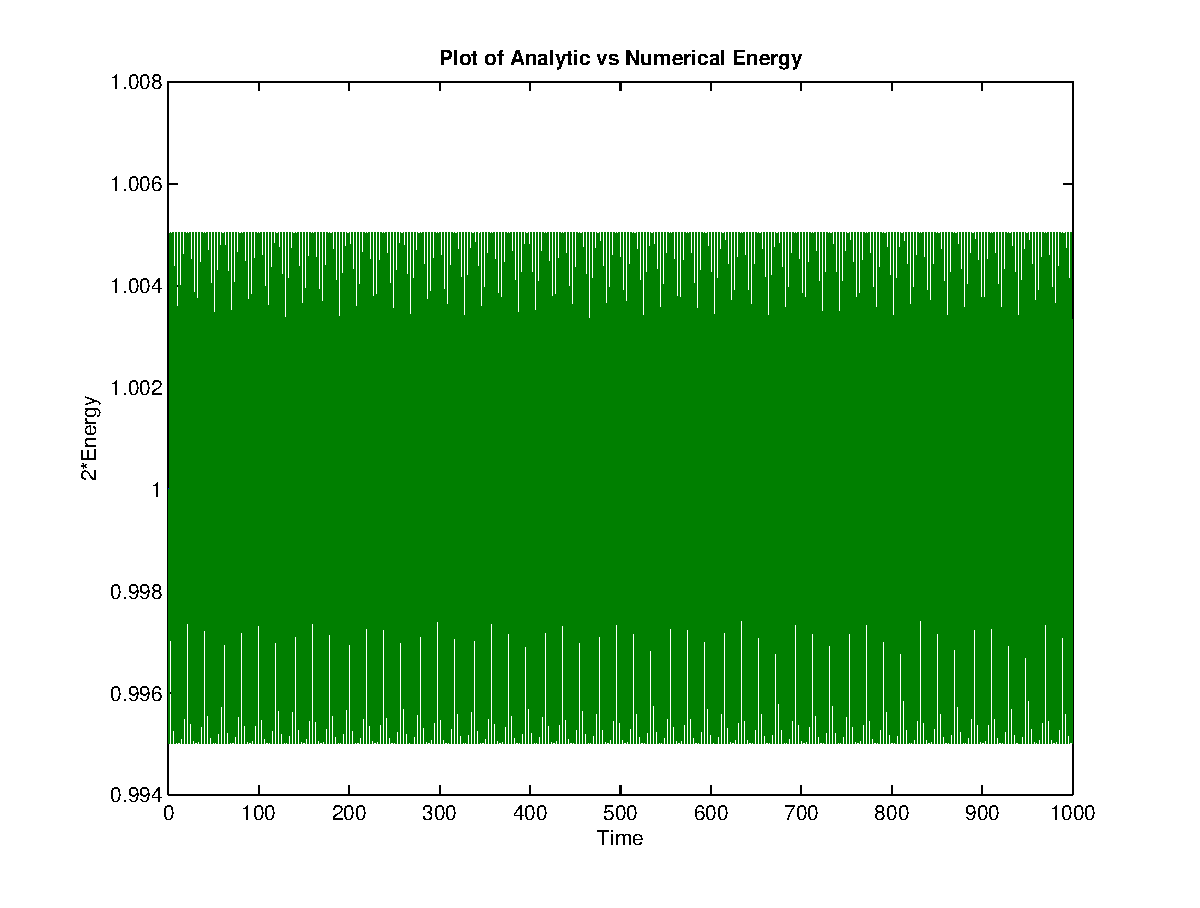
\includegraphics[width=1.1\textwidth]{SymplecticEulerPlotofAnalytVsNumEnergy}
\caption{Plot of the total energy multiplied by 2 of the s.h.o. The exact total energy is in blue, and the symplectic Euler energy is in green.}
\label{fig:figure8}
\end{minipage}
\hspace{0.5cm}
\begin{minipage}[b]{0.45\linewidth}
\centering
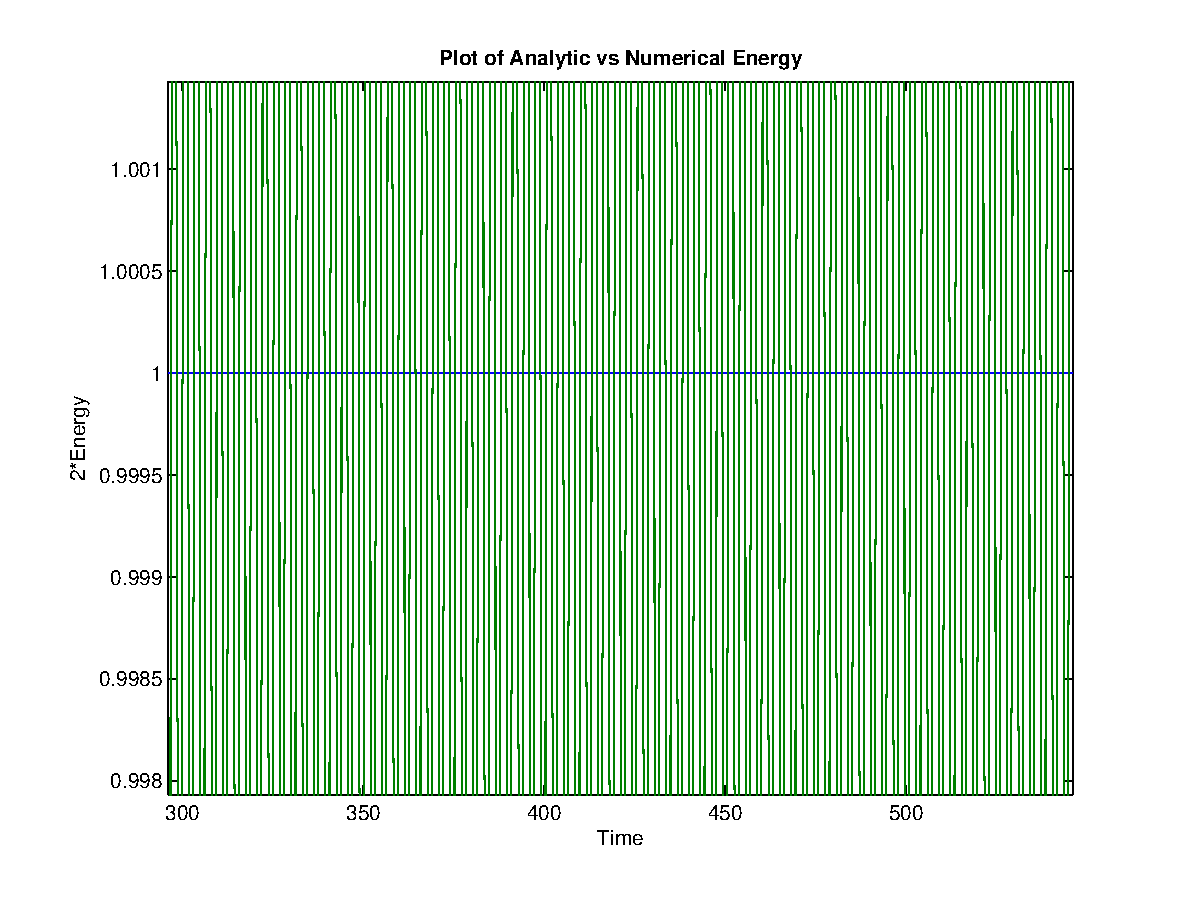
\includegraphics[width=1.1\textwidth]{ZoomedInSymplecticEulerPlotofAnalytVsNumEnergy}
\caption{A close up of the plot of the total energy multiplied by 2 of the s.h.o. showing the high oscillation frequencies near the true value.}
\label{fig:figure9}
\end{minipage}
\end{figure}
\\\\\indent The symplectic Euler has a bounded error for the total energy. The total energy is not conserved, but there is no large increases, and the total energy remains near its true value. Figure 8 and Figure 9 show that the total energy of the symplectic Euler method oscillates very closely to the true value. The magnitude of the computed energy oscilaltes asymmetrically at nearly twice the oscillator frequency about the true energy value with the amplitude of this oscillation related to the time step. So compared to the explicit Euler, the symplectic Euler method has a significant advantage by preserving the underlying geometries, even if there is a small error associated with the time step, the approximation approaches the Hamiltonian we need to solve. 


\section{Second-Order Methods: Second-Order Explicit Runge-Kutta and Velocity Verlet}
We now do a comparison of second order methods, one being the MATLAB ode23 solver which uses simultaneously second and third order Runge-Kutta formulas to make estimates, and the other the symplectic velocity Verlet method. The Runge-Kutta methods that are used in the MATLAB ode23 solver are not symplectic as they are based on a refinement of the explicit Euler method which is not symplectic.
\begin{figure}[h!]
\centering
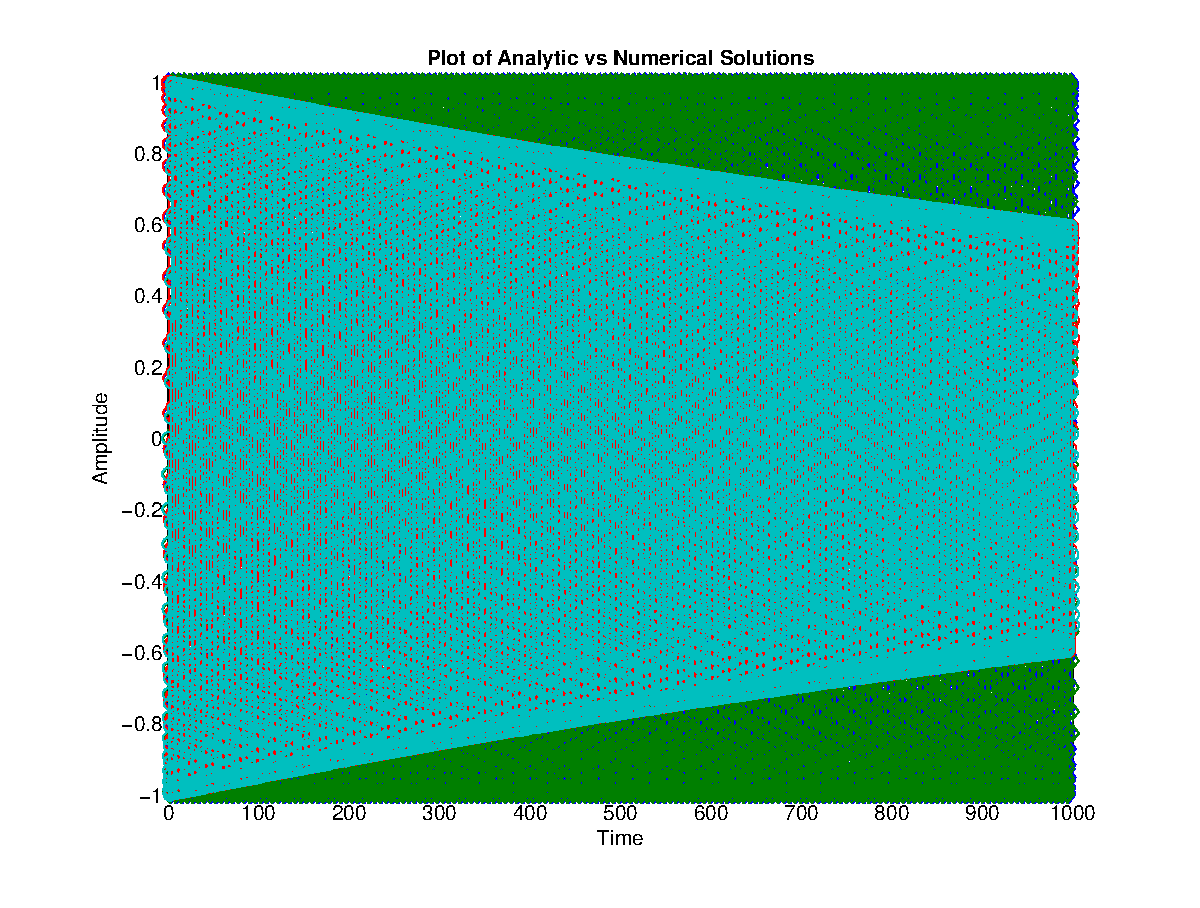
\includegraphics[width=0.675\textwidth]{SecondOrderOde23PlotAnalyticVsNumerSoln}
\caption{Plot of the analytic solution of the s.h.o. q(t) and MATLAB ode23 numerical solution. q(t) is represented by the green and dark blue oscillations that are constant in amplitude over time. MATLAB ode23 solver is represented by the red and the light blue oscillations that are decreasing in amplitude over time.}
\end{figure}
\\\\\indent As we see in Figure 10, as the number of iterations increase, over a long time period the amplitude of the numerical solution is decreasing, rather than staying constant. At the start, the ode23 solver does accurately estimate the solution for about 30 iterations in the time step, but then starts to artificially damp due to the error that is carried from the step size.\\
\begin{figure}[h!]
\centering
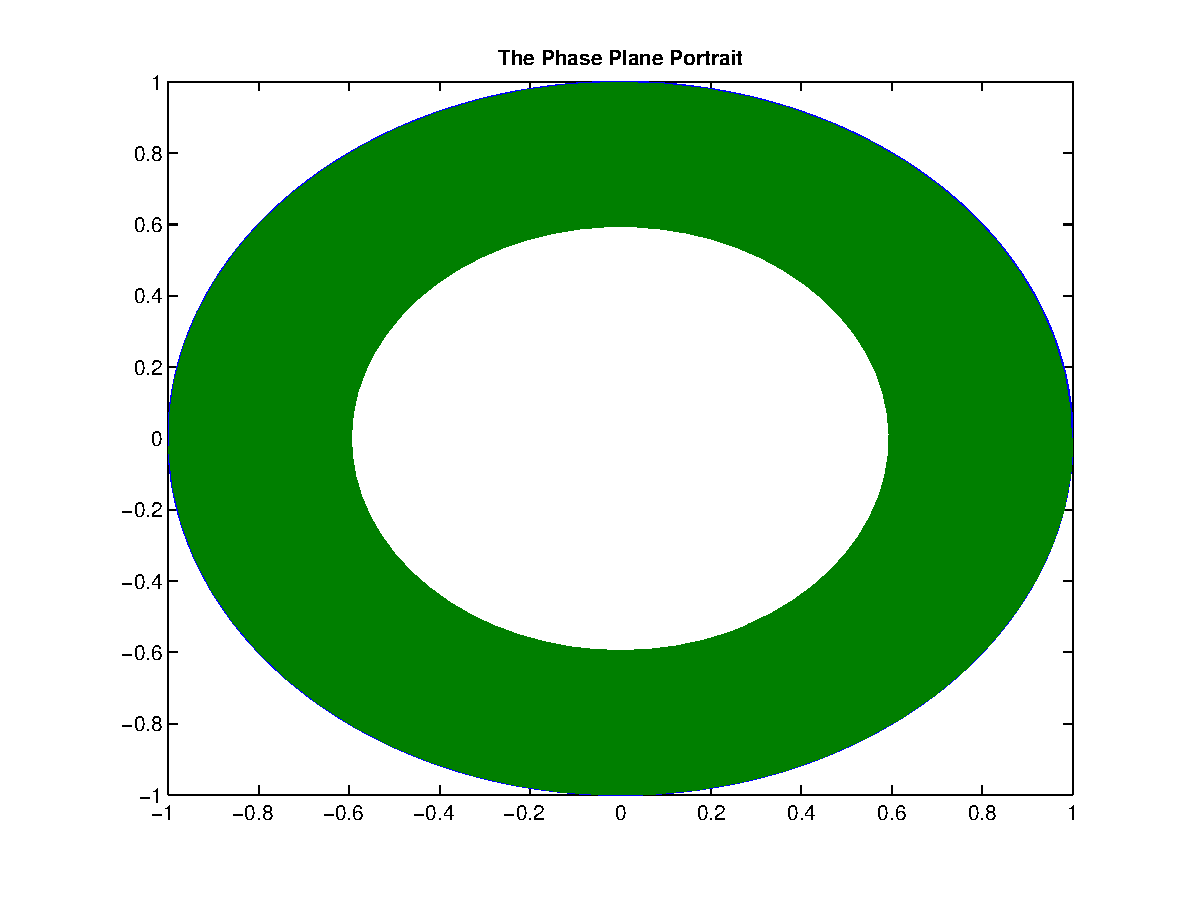
\includegraphics[width=0.675\textwidth]{Ode23SecondOrderPhasePlanePortforSHO}
\caption{Plot of the position-momentum phase space of the MATLAB ode23 solver in green and the exact phase space in blue, which is the exact movement of the s.h.o.}
\end{figure}
\\\\\indent We see that in Figure 11 the ode23 solver does not preserve area in the phase space. Though it initially does a good approximation staying close to the true value of the trajectory, the area in the phase space starts to decrease with each iteration as the trajectory does a very tight spiral inwards towards the center. So, for long time scales it does a poor job in estimating the solution and does not preserve the linear symplectic structure.\\
\begin{figure}[h!]
\centering
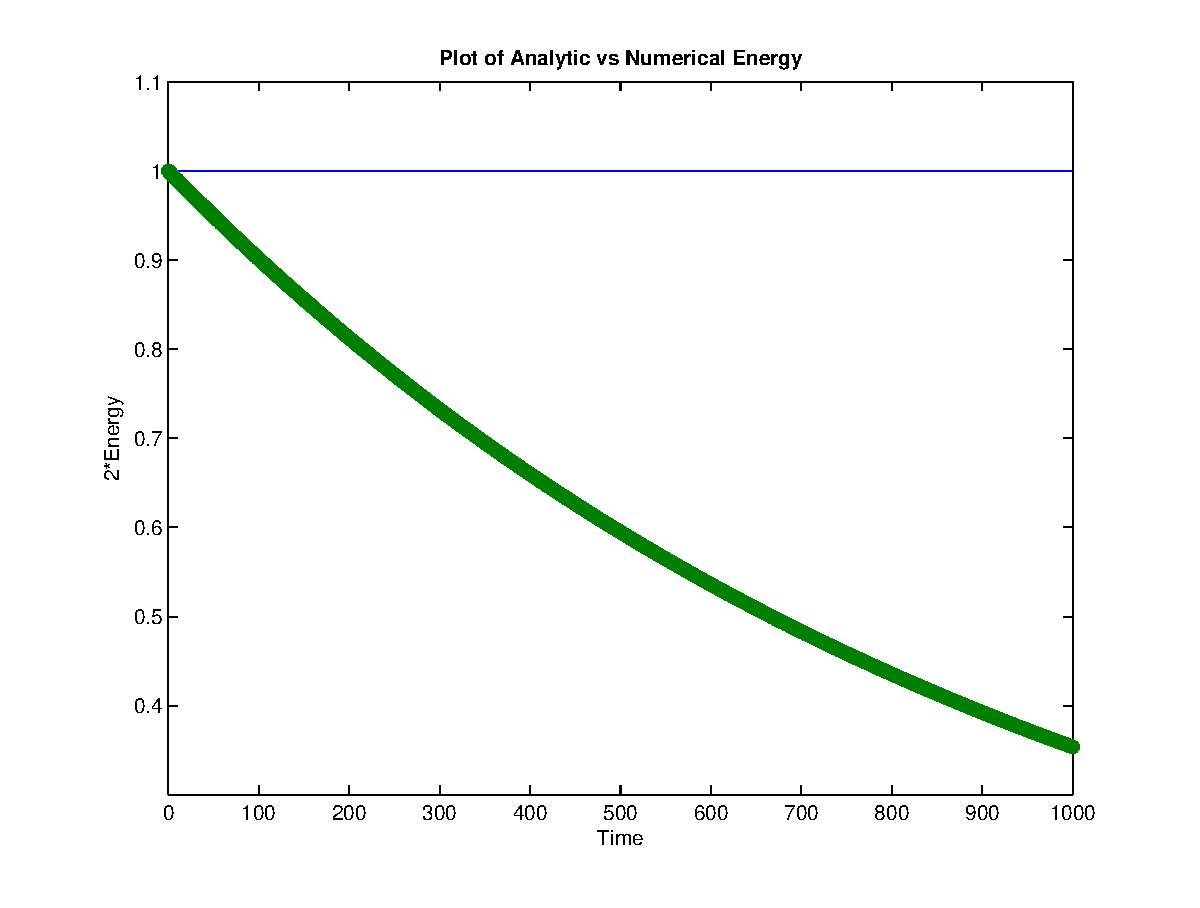
\includegraphics[width=0.675\textwidth]{SecondOrderOde23PlotofAnalytVsNumEnergy}
\caption{Plot of the total energy multiplied by 2 of the s.h.o. in which exact energy is blue and the energy computed by the MATLAB ode23 solver is in green.}
\end{figure}
\\\indent As we can see, the ode23 solver algorithm computed energy deviates more and more from the exact value as time increases, as shown by the green line in Figure 12. The energy monotonically decreases with a factor that closely resembles time step of order 2 (though significantly better than the factor in the explicit Euler method). Now we compare this to the numerical results of the velocity Verlet.\\
\\\indent The velocity Verlet is
\[p_{i+\frac{1}{2}}=p_i+\frac{h}{2}F(q_i)\]
\[q_{i+1}=q_i+hp_{i+\frac{1}{2}}\;\;\]
\[\;\;\;\;\;\;\;\;p_{i+1}=p_{i+\frac{1}{2}}+\frac{h}{2}F(q_{i+1})\]
which can be written for the s.h.o. as
\[q_{i+1}=q_i+hp_i-\frac{1}{2}q_ih^{2}\]
\[p_{i+1}=p_i-\frac{h}{2}(q_i+q_{i+1})\]
To show the velocity Verlet method is symplectic, we write each part of the algorithm as
\[\left (\begin{matrix}
  q_{i}  \\
  p_{i+\frac{1}{2}} 
 \end{matrix}\right)=
\left(\begin{matrix}
  1 & 0 \\
  -\frac{h}{2} & 1 
 \end{matrix}\right)
\left(\begin{matrix}
  q_i  \\
  p_i 
 \end{matrix}\right)\]
letting $\left(\begin{matrix} 1 & 0 \\ -\frac{h}{2} & 1 \end{matrix}\right)=A$ for the first part
\[\left (\begin{matrix}
  q_{i+1}  \\
  p_{i+\frac{1}{2}} 
 \end{matrix}\right)=
\left(\begin{matrix}
  1 & h \\
  0 & 1 
 \end{matrix}\right)
\left(\begin{matrix}
  q_i  \\
  p_{i+\frac{1}{2}} 
 \end{matrix}\right)\]
letting $\left(\begin{matrix} 1 & h \\ 0 & 1 \end{matrix}\right)=B$ for the second part
\[\left (\begin{matrix}
  q_{i+1}  \\
  p_{i+1} 
 \end{matrix}\right)=
\left(\begin{matrix}
  1 & 0 \\
  -\frac{h}{2} & 1 
 \end{matrix}\right)
\left(\begin{matrix}
  q_{i+1}  \\
  p_{i+\frac{1}{2}} 
 \end{matrix}\right)\]
letting $\left(\begin{matrix} 1 & 0 \\ -\frac{h}{2} & 1 \end{matrix}\right)=C$ for the third part. Thus combining everything we get
\[\left (\begin{matrix}
  q_{i+1}  \\
  p_{i+1} 
 \end{matrix}\right)=J\left(\begin{matrix}
  q_{i}  \\
  p_{i} 
 \end{matrix}\right)\]
where $J$ is the Jacobian and is given by the matrix product $J=CBA$. From this we use the theorem that if we have a determinant of a matrix product then we have a product of determinants $\text{det}J$=$\text{det}C$ $\text{det} B$ $\text{det} A$. By inspection, $\text{det} C=\text{det} B=\text{det} A=1$, so that $\text{det} J$ is equal to unity. Thus, velocity Verlet method is symplectic.\\
\begin{figure}[h!]
\begin{minipage}[b]{0.45\linewidth}
\centering
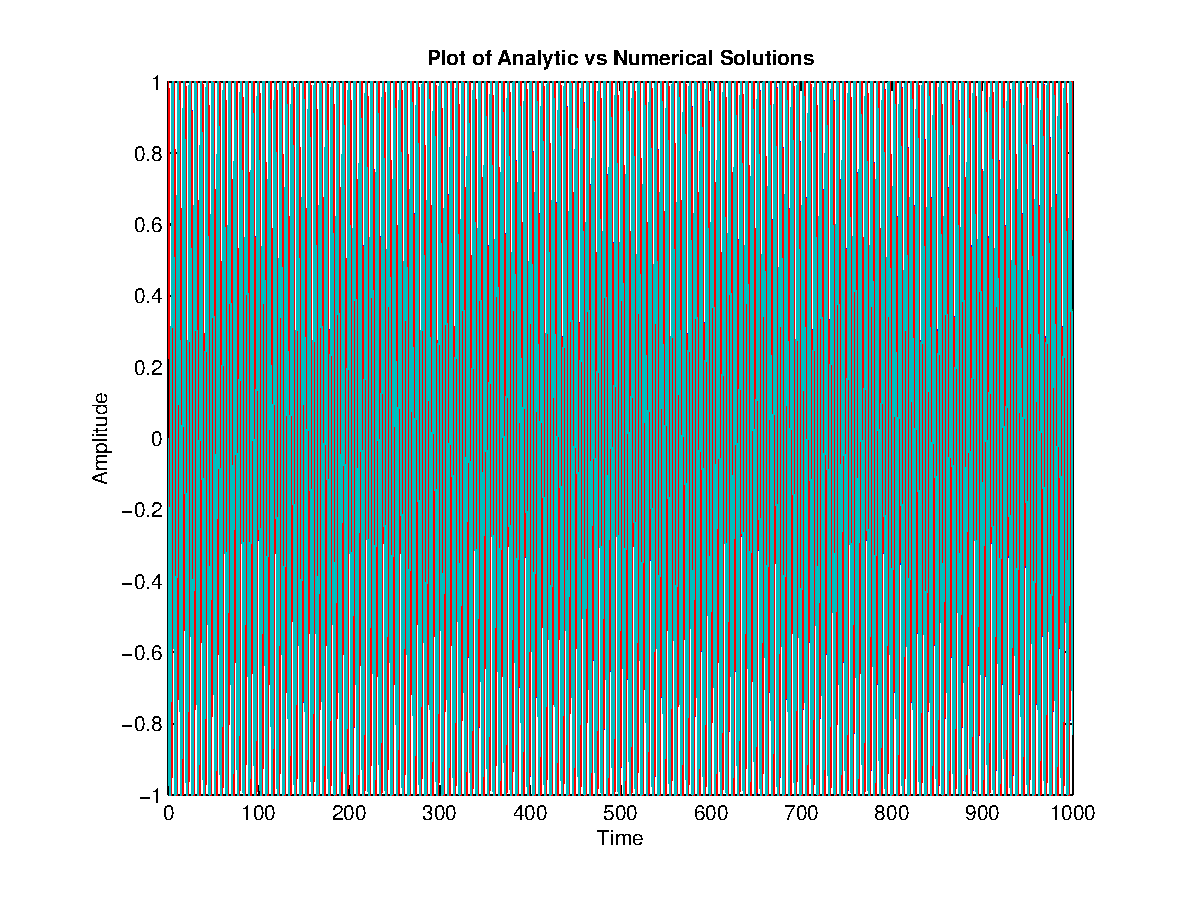
\includegraphics[width=\textwidth]{VelocityVerletPlotofAnalyVsNumSoln}
\caption{Plot of the analytic solution $q(t)$ of the s.h.o. in green and dark blue and plot of the velocity Verlet numerical solution in red and light blue}
\label{fig:figure13}
\end{minipage}
\hspace{0.5cm}
\begin{minipage}[b]{0.45\linewidth}
\centering
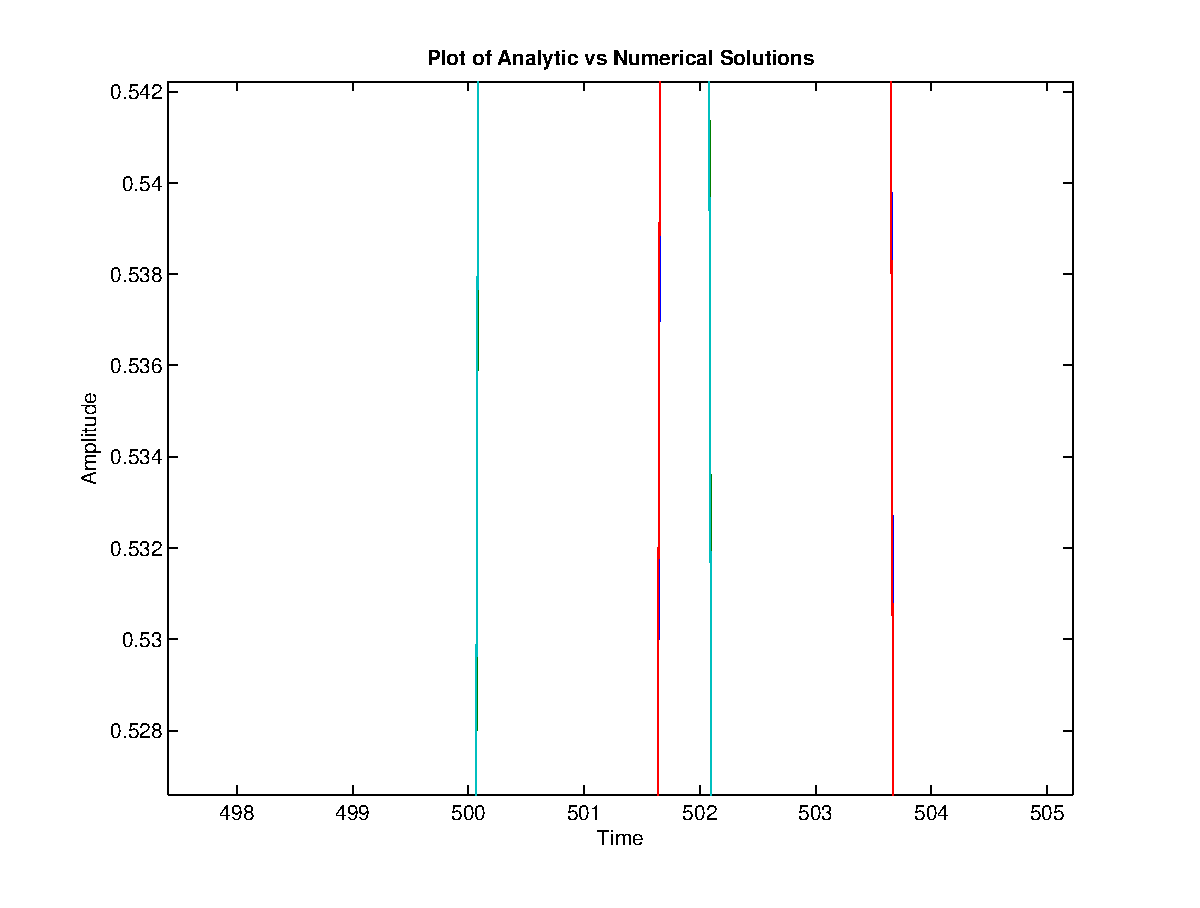
\includegraphics[width=\textwidth]{ZoomedInVelocityVerletPlotofAnalytVsNumSoln}
\caption{A close-up of the plot in Figure 13. Here we can see the strong approximation of the velocity Verlet method in relation to the exact solution.}
\label{fig:figure14}
\end{minipage}
\end{figure}
\\\\\indent We see in Figure 13 and Figure 14 that the numerical approximation done by the velocity Verlet method is very close to the exact solution. The velocity Verlet method is very similar to that of the symplectic Euler, except the half time step gives the velocity Verlet an added order, making it more accurate in the longer time scales. Figure 5 shows that even though the approximation is quite good, it is not exact (not a perfectly overlap). It seems that the velocity Verlet, much like the symplectic Euler, approximates the s.h.o. by essentially solving a small perturbated s.h.o. system that is quite similar to the s.h.o. The velocity Verlet method does this with better error approximation versus the symplectic Euler, and is clearly already better in the long time scales than ode23 solver.
\begin{figure}[h!]
\begin{minipage}[b]{0.45\linewidth}
\centering
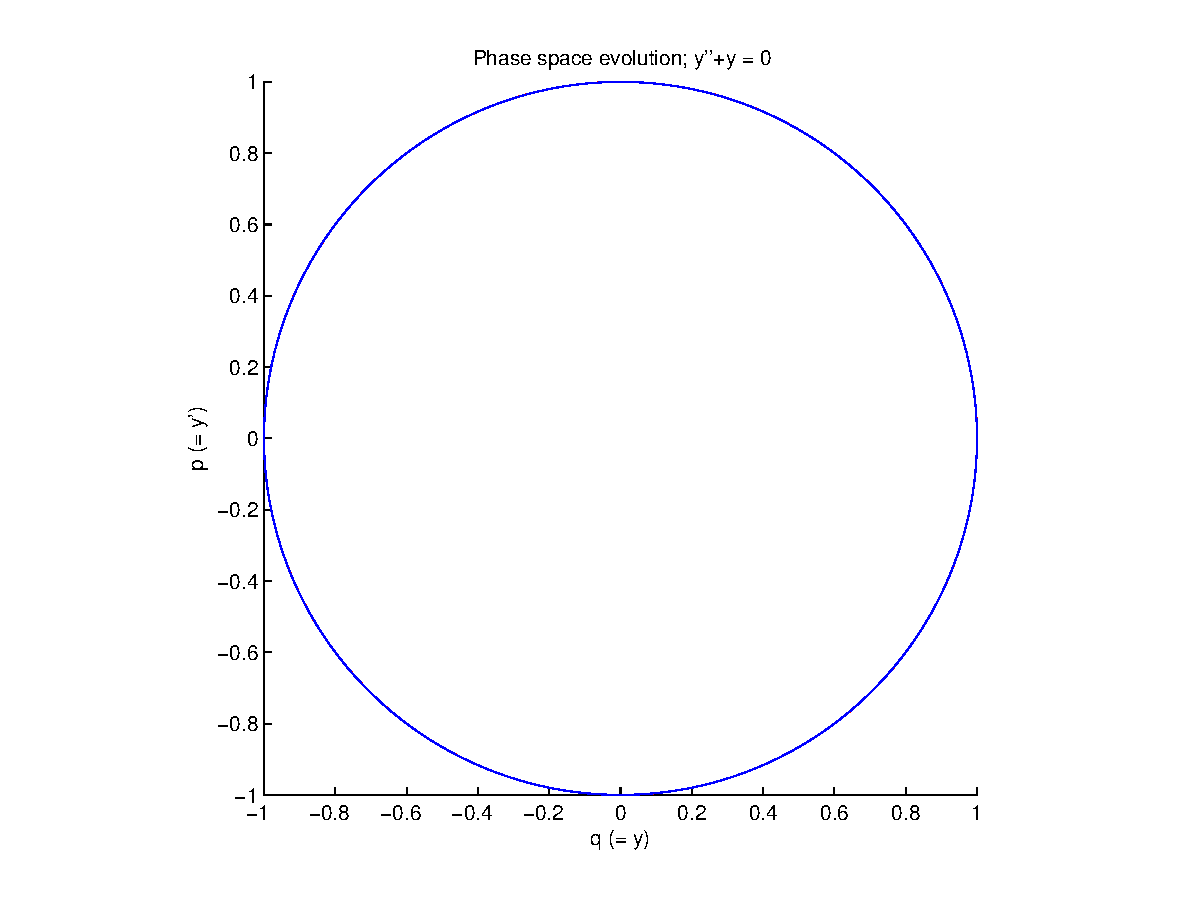
\includegraphics[width=1.1\textwidth]{VelocityVerletPhaseSpacePlot}
\caption{Plot of the position-momentum phase space of the velocity Verlet method in red and the exact phase space in blue.}
\label{fig:figure15}
\end{minipage}
\hspace{0.5cm}
\begin{minipage}[b]{0.45\linewidth}
\centering
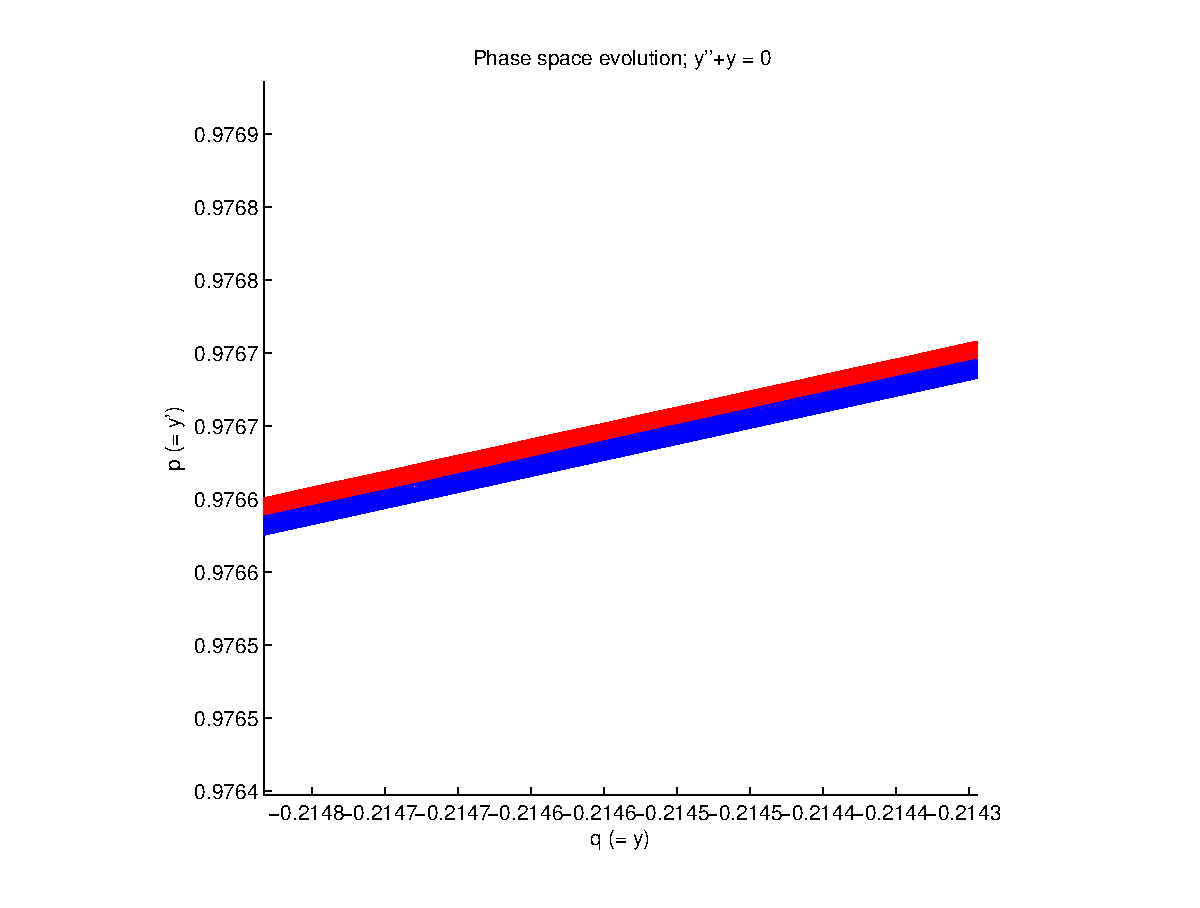
\includegraphics[width=1.1\textwidth]{ZoomedInVelocityVerletPhaseSpacePlot}
\caption{A close-up of the plot of the position-momentum phase space showing the very slight difference of approximation solution.}
\label{fig:figure16}
\end{minipage}
\end{figure}
\\\\\indent   The velocity Verlet method preserves the area in the phase space as the trajectory goes in a circular motion, as seen in Figure 15. The close-up in Figure 16 shows that like the symplectic Euler method, velocity Verlet scheme preserves the area in the phase space of a trajectory of a modified Hamiltonian system that is equal to a small perturbed s.h.o. system, which occurs from the approximation in the time step for each iteration. As we take smaller and smaller time steps, we will approach the exact Hamiltonian of the s.h.o. thereby getting better and better overlap of the exact phase space with the numerically calculated phase space. As seen in Figure 16, the approximation is quite tightly packed near the true phase space trajectory.
\begin{figure}[h!]
\centering
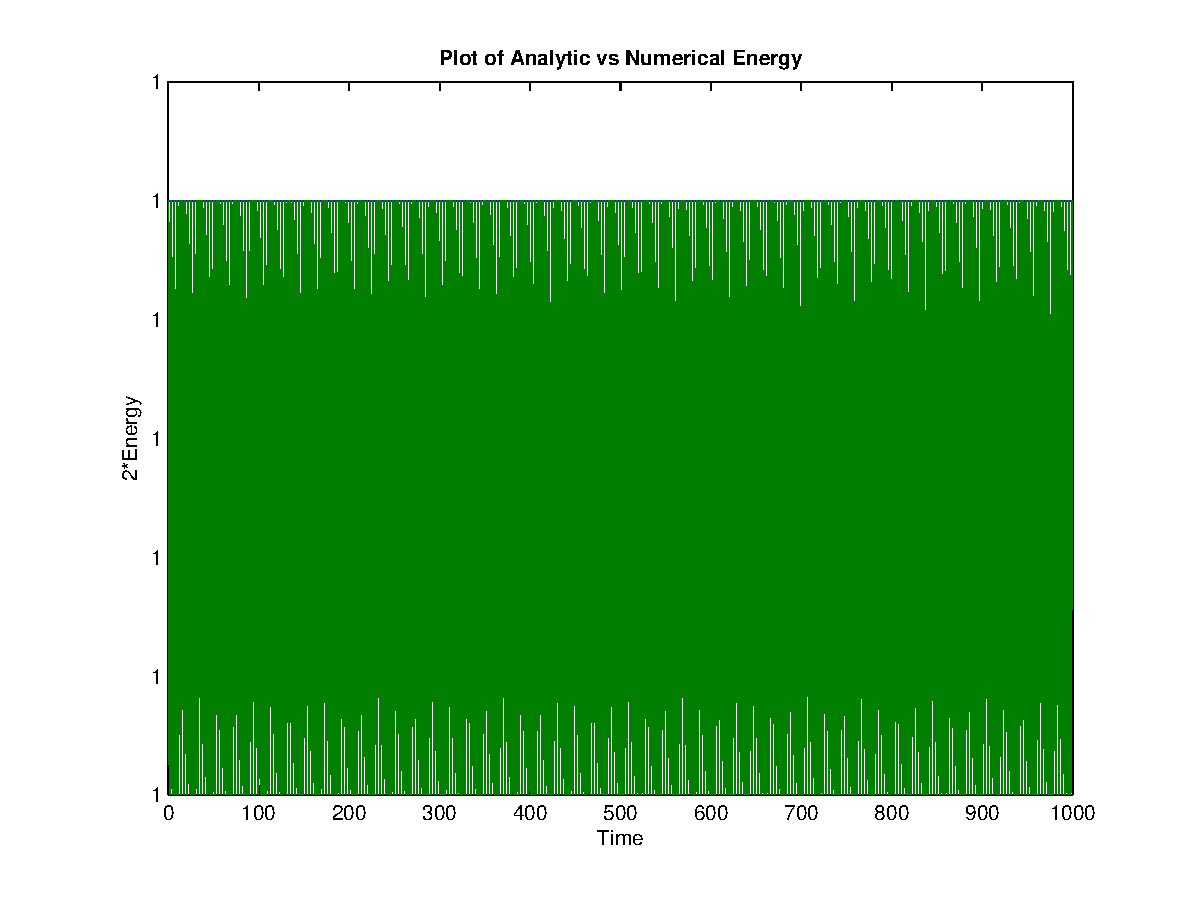
\includegraphics[width=0.64\textwidth]{VelocityVerletPlotofAnalytVsNumEnergy}
\caption{Plot of the total energy multiplied by 2 of the s.h.o. in which exact energy is blue and the energy computed by the velocity Verlet method is in green.}
\end{figure}
\\\indent The energy approximation computed by the velocity Verlet method essentially oscillates very closely around the the true energy value, with global error bound of order two. The y-scale shows that the oscillations are very well approximated closely to the true value. The approximation is significantly better than the algorithms we have seen thus far. It can be noted that the long-term results of velocity Verlet are one order better than symplectic Euler. The algorithms are almost identical up to a shifted by half of a time step in the velocity. It's suprising how that shift in the time step for velocity created a significant efficiency in the algorithm and also had a much better approximation while perserving the symplectic structure. 


\section{Fourth-Order Methods: Fourth-Order Explicit Runge-Kutta and Forest-Ruth}
MATLAB ode45 solver is the most common general purpose o.d.e. solver used in numerical analysis. Fourth-order methods generally are the most useful higher-order approximations due to the relative computational speed of the algorithm and the efficiency. Anything higher might create complexities that are unnecessary burden to running an estimation. There are many fourth-order symplectic methods, I chose one that was studied by Forest and Ruth \cite{ER}, but other fourth-order methods exist such as the one developed in \cite{CR}.\\\\
\indent The MATLAB ode45 solver uses fourth and fifth order Runge-Kutta (RK) formulas to make error estimates and adjust the time step accordingly. As we will see, this particular method is not symplectic. It can be verified that the RK formulas used for ode45 solver do not satisfy the condition of an algorithm being symplectic. \\\\
\indent We see in Figure 18 that the ode45 solver does a decent approximation for a long period of time, compared to the other general o.d.e. solvers. Though, for very long time scales, the accuracy cannot be compensated for, and thus the amplitude of the oscillations very slowly decreases over time for each iteration rather than being constant like the exact solution. Though this approximation is quite good for a method that is not symplectic.\\
\begin{figure}[h!]
\centering
\includegraphics[width=0.675\textwidth]{FourthOrderOde45PlotofAnalytVsNumSoln}
\caption{Plot of the analytic solution of the s.h.o. q(t) and MATLAB ode45 numerical solution. q(t) is represented by the green and dark blue oscillations that are constant in amplitude over time. The red and the light blue oscillations that are decreasing in amplitude over time represent the explicit Euler method.}
\end{figure}
\\\indent Like the ode23 solver, the ode45 solver also spirals inwards towards the center for the phase space trajectory, as shown in Figure 19. The inward spiral of the trajectory is much slower due to the error control of the ode45 is much better (order 4/5), hence why does better in comparison to ode23. For the first thousand time steps it holds fairly tightly to the true value, but then becomes more apparently diverging inwards away from the true value. \\
\begin{figure}[h!]
\centering
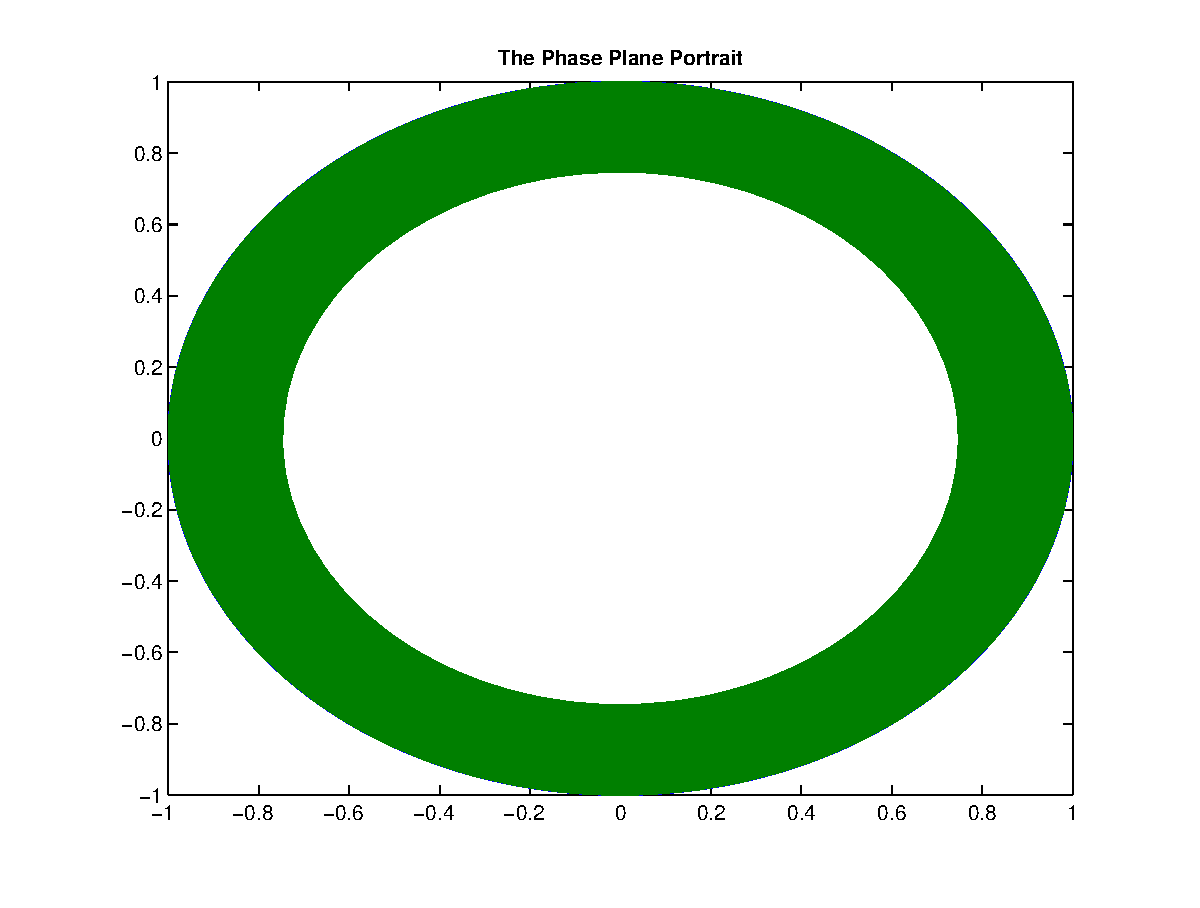
\includegraphics[width=0.675\textwidth]{FourthOrderOde45PhasePlanePlot}
\caption{Plot of the position-momentum phase space of the MATLAB ode45 solver in green and the exact phase space in blue, which is the exact movement of the s.h.o.}
\end{figure}
\\\\\\\\\indent Lastly, the plot of the total energy in Figure 20 shows that the ode45 solver monotonically decreasing away from the true value, towards zero. From the graph, it is doing this at a much slower rate (the slope comparison) than ode23 solver obviously, slowly increasing the error with each iteration diverging from the constant value. 
\begin{figure}[ht]
\centering
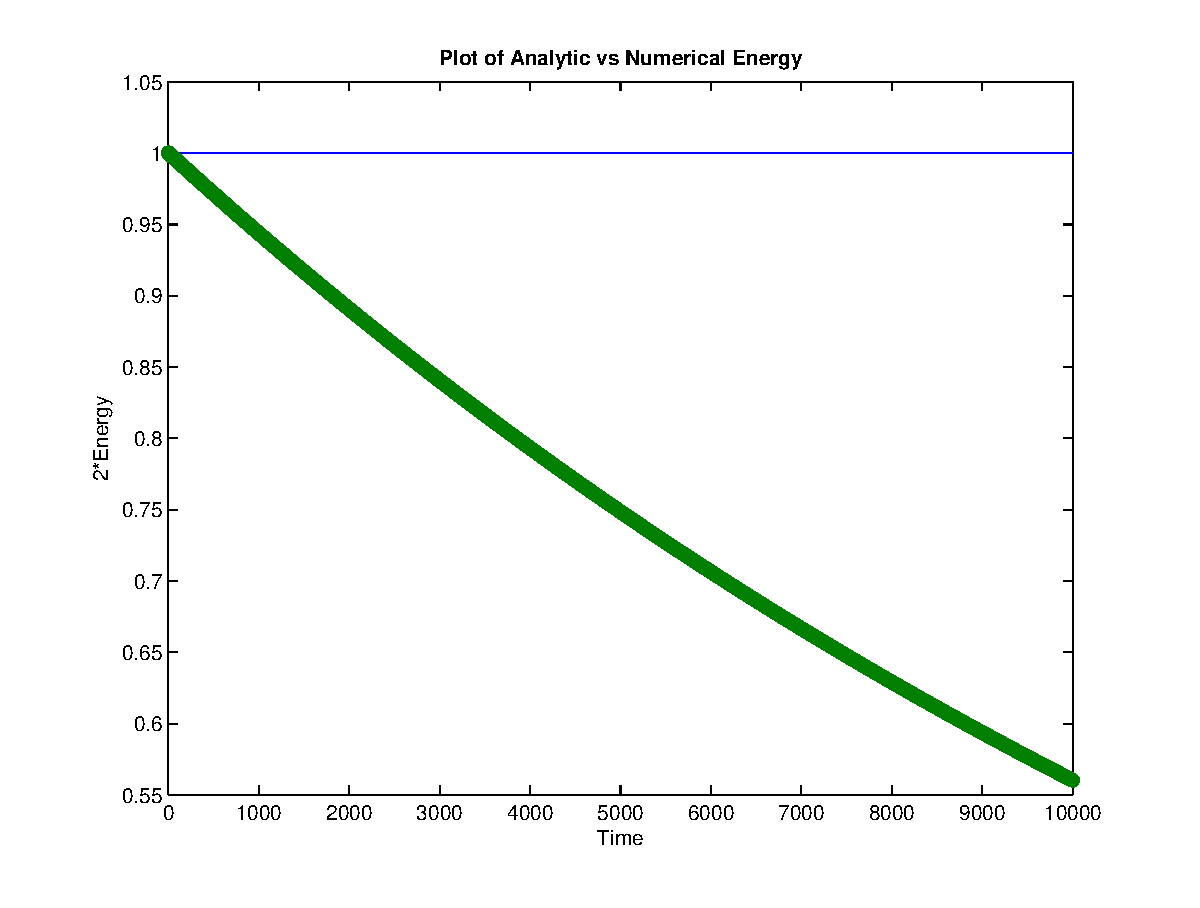
\includegraphics[width=0.675\textwidth]{FourthOrderOde45AnalytVsNumEnergyPlot}
\caption{Plot of the total energy multiplied by 2 of the s.h.o. in which exact energy is blue and the energy computed by the MATLAB ode45 solver is in green.}
\end{figure}
Now, we compare this to the Forest-Ruth Algorithm (FR4) that is a symplectic integrator of fourth-order originally constructed in \cite{ER}. \\
\\\indent The FR4 method is the simplest higher order symplectic algorithm and is constructed as follows, we let velocity be equal to the momentum $p$ with $m=1$
\[q_{i+1}=q_{i}+\theta \frac{h}{2}p_i\]
\[\;\;\;\;\;\;\;\;p_{i+1}=p_{i}+\theta hF(q_{i+1})\]
\[\;\;\;\;\;\;\;\;\;\;\;\;\;\;\;\;q_{i+1}=q_{i+1}+(1-\theta) \frac{h}{2}p_{i+1}\]
\[\;\;\;\;\;\;\;\;\;\;\;\;\;\;\;\;\;\;\;\;\;\;\;p_{i+1}=p_{i+1}+(1-2\theta) hF(q_{i+1})\]
\[\;\;\;\;\;\;\;\;\;\;\;\;\;\;\;\;\;q_{i+1}=q_{i+1}+(1-\theta) \frac{h}{2}p_{i+1}\]
\[\;\;\;\;\;\;\;\;\;\;\;\;\;p_{i+1}=p_{i+1}+\theta hF(q_{i+1})\]
\[\;\;\;\;\;\;\;\;\;q_{i+1}=q_{i+1}+\theta \frac{h}{2}p_{i+1}\]
with 
\[\theta=\frac{1}{{2-\sqrt[3]{2}}}\]
Thus this is the FR4 algorithm to generate one time step. Note that this method requires three evaluations of the force per time step. Note that the steps are symmetric about the middle step. To show symplecticity, we see that since each step is simply moving forward either the position or the velocity (momentum p), the Jacobian of the transformation can be written as a product of determinants (we have 7 here), each of which trivially has determinant equal to unity. Hence FR4 is symplectic. In \cite{ER}, they show that the algorithm gives an error of order ${h}^{5}$ for one interval (and hence of order ${h}^{4}$ when integrated over n=T/h time steps for a fixed time increment T), which gives rise to the value $\theta$. \\
\begin{figure}[h!]
\begin{minipage}[b]{0.45\linewidth}
\centering
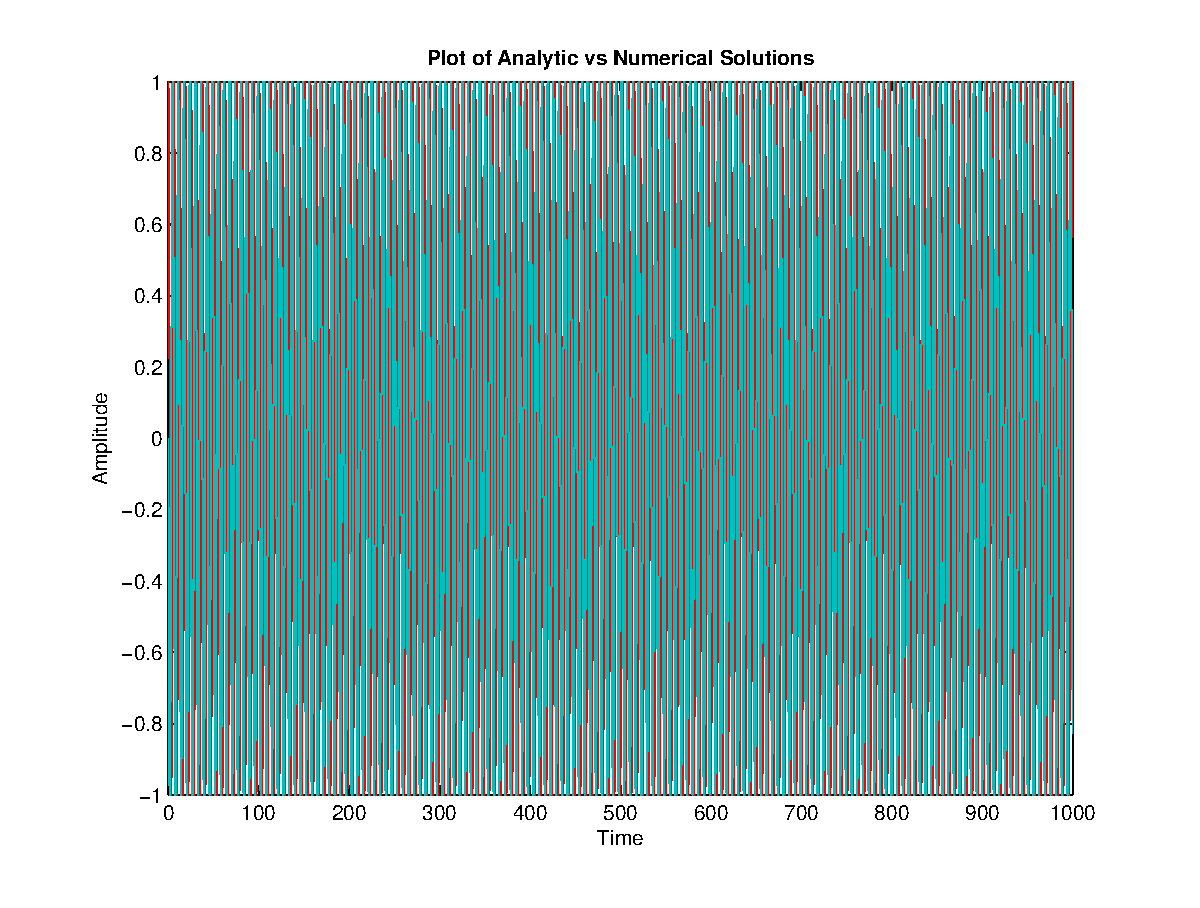
\includegraphics[width=1.1\textwidth]{SymplecticFourthOrderPlotOfAnalytVsNumSoln}
\caption{Plot of the analytic solution $q(t)$ of the s.h.o. in green and dark blue and plot of the FR4 numerical solution in red and light blue}
\label{fig:figure21}
\end{minipage}
\hspace{0.5cm}
\begin{minipage}[b]{0.45\linewidth}
\centering
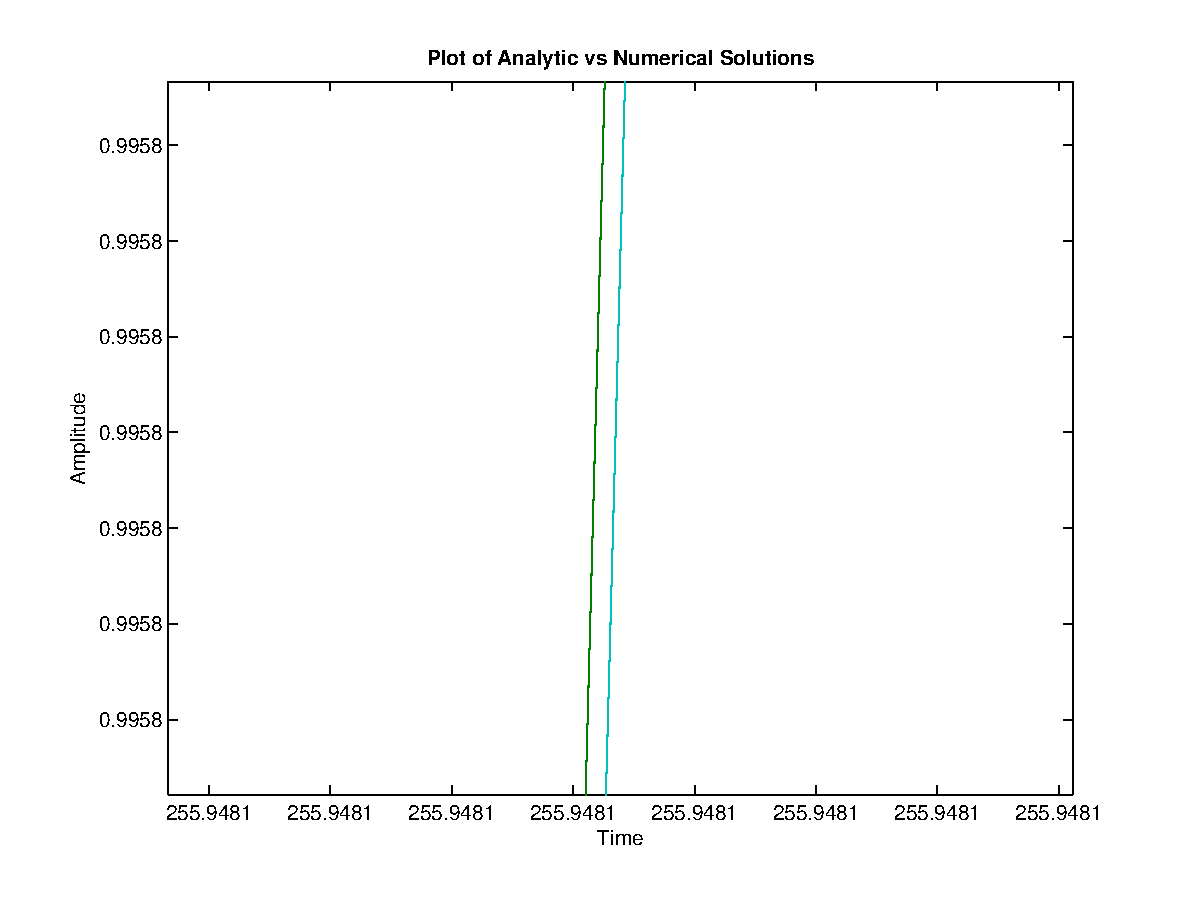
\includegraphics[width=1.1\textwidth]{ZoomedInFourthOrderPlotofAnalyVsNumSoln}
\caption{A close-up of the plot in Figure 21. Here we can see the strong approximation of the velocity Verlet method in relation to the exact solution.}
\label{fig:figure22}
\end{minipage}
\end{figure}
\\\indent We see in Figure 21 that the approximated solution via FR4 has extremely good overlap with the exact solution, meaning the error per iteration is very low and stays quite near to the true value. It can be seen in Figure 22 that the approximation is not quite exact, but it extremely close to the true values, giving much better truncation error per time step than all other methods seen thus far (order 4 versus order 2 from velocity Verlet). We can appreciate just how good the approximation is by zooming in to the oscillations and noting that even though there is no perfect overlap, the distinction of the approximation can only be seen for very very small time intervals, and even then the approximate value values differ at a scale smaller than the magnitude of $10^{-4}$ that is being displayed in the graph.\\
\begin{figure}[h!]
\begin{minipage}[b]{0.45\linewidth}
\centering
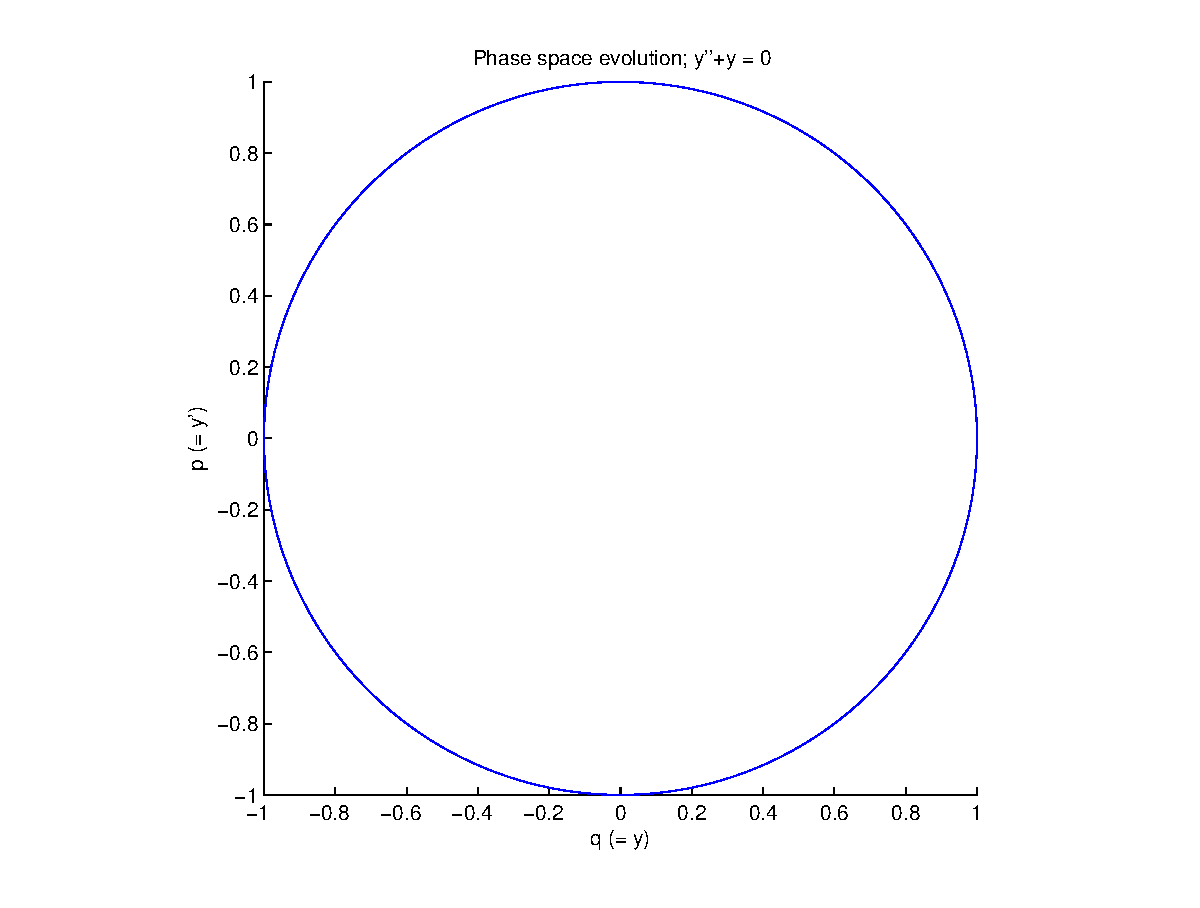
\includegraphics[width=1.1\textwidth]{SymplecticFourthOrderPhaseSpacePlot}
\caption{Plot of the position-momentum phase space of the FR4 method in red and the exact phase space in blue.}
\label{fig:figure23}
\end{minipage}
\hspace{0.5cm}
\begin{minipage}[b]{0.45\linewidth}
\centering
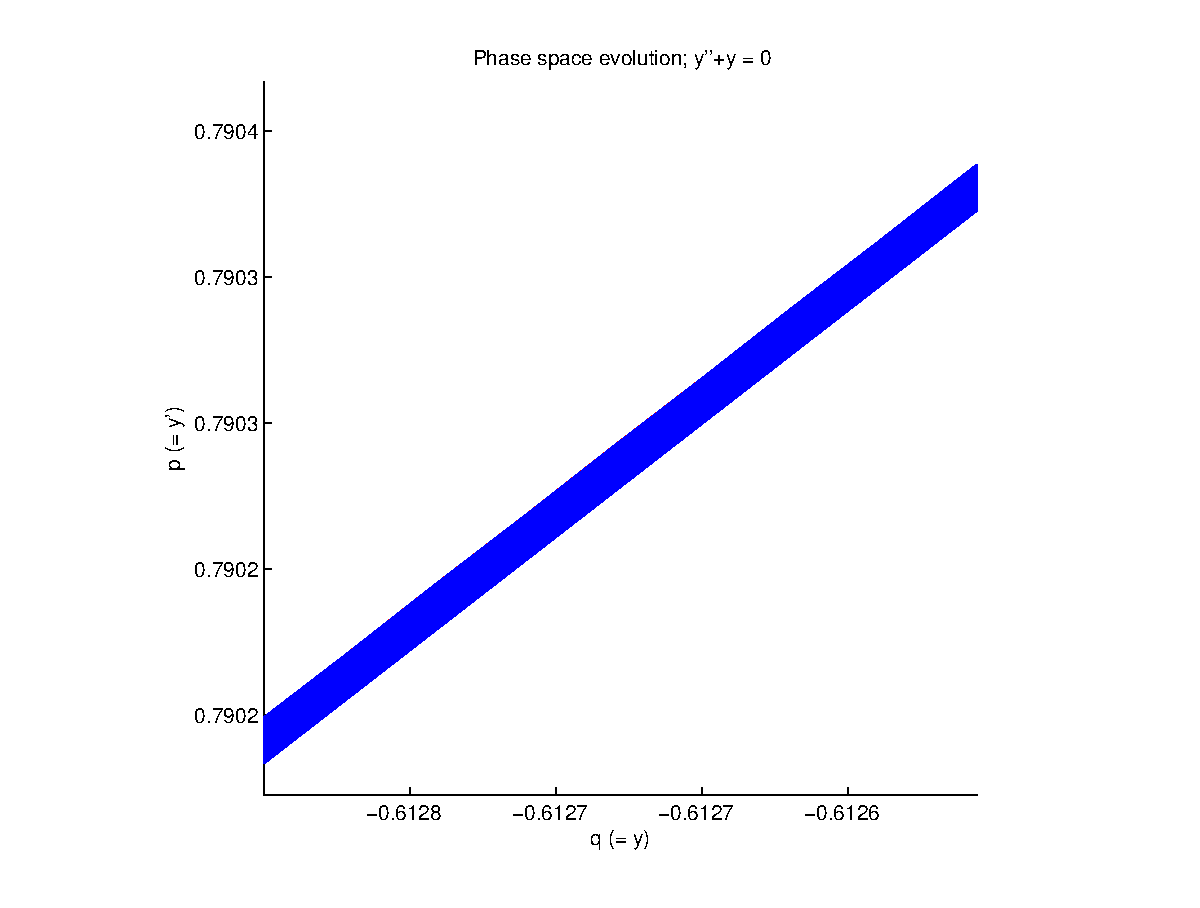
\includegraphics[width=1.1\textwidth]{ZoomedInSymplecticFourthOrderPhaseSpacePlot}
\caption{A close-up of the plot of the position-momentum phase space showing the very slight difference of approximation solution.}
\label{fig:figure24}
\end{minipage}
\end{figure}
\\\indent We see in Figure 23 that the approximation done by the FR4 method is overlapped with the exact phase space trajectory. Clearly it preserves the area in the phase space. A close-up of the plot, in Figure 24, shows how tightly bounded the error is as it approached the exact phase space trajectory by solving a modified Hamiltonian of the s.h.o. It is extremely difficult to see any of the red line which represents the numerical approximation as the approximation is very near to the true value. The FR4 does a superb job in modeling the trajectory and thus the movement of the harmonic oscillator (even if it models an extremely small perturbation of the system). It is seen that over long time scales, the FR4 method essentially approaches the exact Hamiltonian of the s.h.o.
\begin{figure}[h!]
\centering
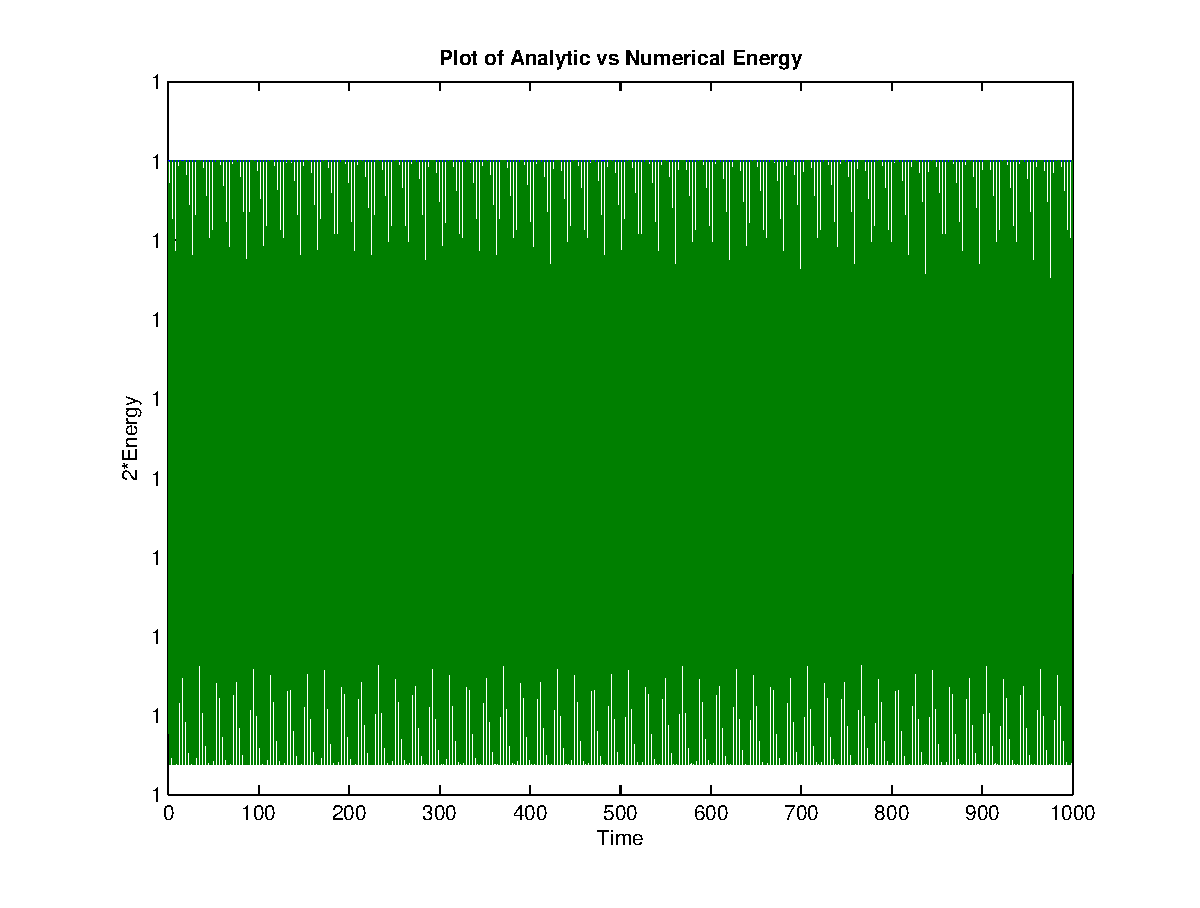
\includegraphics[width=0.50\textwidth]{SymplecticFourthOrderPlotofAnalyVsNumEner}
\caption{Plot of the total energy multiplied by 2 of the s.h.o. in which exact energy is blue and the energy computed by the FR4 method is in green.}
\end{figure}
\\\indent We see in Figure 25 that the FR4 computed energy oscillates very closesly to the true value of the system, shown in blue at the very top of the green high frequency oscillations (which represent the numerical approximations for each time step). The accuracy of the algorithm is very good as such methods have global stability for very long time scales. By comparing the errors with the velocity Verlet, one can see, as expected, that the error in velocity Verlet varies in ${h}^{2}$, while that in FR4 varies as ${h}^{4}$. Clearly, this method can be seen to be much closer to the true system as the number of iterations increases, with the each time step the modified Hamiltonian that FR4 solves for will approach the true Hamiltonian values much faster and with better accuracy than the velocity Verlet method (and clearly better than all other methods stated and compared). 


\section{Conclusion}
The advantage of symplectic algorithms is that they possess global stability. Since the area bounded by adjacent trajectories is preserved, there will not be a situation where the coordinates (and hence the energy) increase without bound (explicit Euler), because this would expand the area. Even in better non-symplectic approximations, such as ode23 solver (RK2/3) and ode45 solver (RK4/5), the energy will deviate substantially from its initial value at sufficiently long times.\\\\
\indent A symplectic integrator will represent the exact solution of some Hamiltonian. However, it will not be the exact Hamiltonian. It will be a modified Hamiltonian such that as you take smaller and small time steps, the symplectic integrator will solve a problem that is closer and closer to the actual problem you are interested in. For the symplectic integration scheme there is a good connection to conservation of energy. However, the energy conserved by the symplectic numerical method will in general be different from the energy of the original system being analyzed. But, for a good numerical method, the perturbed energy should be close to the exact conserved energy of the system. In many applications, the most noticeable features of the solutions appear only after long times or large number of iterations. In these applications, false damping or excitation may lead to misleading results, thereby requiring the symplectic integrator algorithm. \\\\
\indent Even though symplectic integrators are quite advantageous, a small caution needs to be taken. If the forces involved in a system are particularly small a portion of the time, so having changes in velocity that are small in this region, but forces are very large at other times, then one would like to be able to change the stepsize $h$ during the run (adaptive stepsize control). In this way one could make large strides during the time in which not much is happening, but then go on a fine mesh of time steps in regions where the rate of velocity change is large. Adaptive stepsize control has been implemented in RK4 and similar methods. Though RK4 method is quite accurate, they are not symplectic as we have seen. It might be wise to use RK4 with adaptive stepsize control when dealing with large variations in the force, rather than symplectic algorithms with no adaptive stepsize control.


\newpage
\begin{thebibliography}{1}

  \bibitem{DR} D. Donnelly and E. Rogers, \emph{Symplectic Integrators: An Introductions}, Am. J. Phys. 73, 938 (2005).

  \bibitem{EH} Ernst Hairer, \emph{Lecture 2: Symplectic Integrators}, \url{http://www.unige.ch/~hairer/poly_geoint/week2.pdf}

  \bibitem{ER} E. Forest and R.D. Ruth, \emph{Fourth-Order Symplectic Integration}, Physica D, 43, 105 (1990)

  \bibitem{CR}  J. Candy and W. Rozmus, \emph{A symplectic integration algorithm for separable
Hamiltonian functions}, J. Comput. Phys. 92 (1991), no. 1, 230-256.

  \bibitem{CS} P. J. Channell and C. Scovel, \emph{Symplectic integration of Hamiltonian systems}, Nonlinearity 3 (1990), no. 2, 231-259.

  \bibitem{MPS} J. E. Marsden, G. W. Patrick, and W. F. Shadwick (eds.), \emph{Integration algorithms and classical mechanics}, American Mathematical Society, Providence, RI, 1996.

  \bibitem{RR} R. D. Ruth, \emph{A canonical integration technique}, IEEE Trans. Nucl. Sci. 30
(1983), 2669-2671.

  \bibitem{RV} R. de Vogelaere, \emph{Methods of integration which preserve the contact transformation porperty of hamiltonian equations}, Tech. Report No 4, Dept. Mathem., Univ. of Notre Dame, Notre Dame, Ind., 1956.

\end{thebibliography}

\end{document}